\documentclass[output=paper
,modfonts
,nonflat,draftmode]{langsci/langscibook} 
%\bibliography{mwe2017bib3}
%% add all extra packages you need to load to this file 
\usepackage{graphicx}
\usepackage{tabularx}
\usepackage{amsmath} 
\usepackage{multicol}
\usepackage{lipsum}
%%%%%%%%%%%%%%%%%%%%%%%%%%%%%%%%%%%%%%%%%%%%%%%%%%%%
%%%                                              %%%
%%%           Examples                           %%%
%%%                                              %%%
%%%%%%%%%%%%%%%%%%%%%%%%%%%%%%%%%%%%%%%%%%%%%%%%%%%%
% remove the percentage signs in the following lines
% if your book makes use of linguistic examples
\usepackage{langsci/styles/langsci-gb4e} 
\usepackage{langsci/styles/langsci-optional} 
\usepackage{langsci/styles/langsci-lgr}
\usepackage{langsci/styles/langsci-bidi}
\usepackage{morewrites} 
%% if you want the source line of examples to be in italics, uncomment the following line
% \def\exfont{\it}

%\usepackage{enumitem} %Conflict with enumerate
\usepackage{lipsum}
\usepackage{multirow}
\usepackage{graphicx}
\usepackage{epstopdf}
\usepackage{wrapfig}
\usepackage{caption}
\usepackage{subcaption}
\usepackage{url}
\usepackage{relsize}
\usepackage{paralist}
\usepackage{tabularx} 
%\newfontfamily\Parsifont[Script=Arabic]{langsci/fonts/ScheherazadeRegOT_Jazm.ttf} 
\usepackage{latexsym}
\usepackage{tikz-dependency}
\usepackage{textgreek}
\usepackage{color}
\usepackage{newfloat}
\usepackage{hhline}
\usepackage{xspace}
\usepackage{booktabs}
\usepackage{verbatim} 
\usepackage{algorithm}
\usepackage[noend]{algpseudocode}
\usepackage{sidecap}
\usepackage{kantlipsum}
\usepackage{verbatimbox} 
\usepackage[usestackEOL]{stackengine}
\usepackage{tikz}
\usetikzlibrary{shapes.arrows}
\usepackage{todonotes}
\usepackage{csquotes}
\usepackage{amsmath}
%\usepackage[british]{babel}
\usepackage{mathtools}  % better amsmath
\usepackage{dcolumn}
\newcolumntype{d}[0]{D{.}{.}{2}}
\usepackage{cjhebrew} % Hebrew
\usepackage[normalem]{ulem}
\usepackage{qtree}
\usepackage{rotating}
\usepackage[section]{placeins} 
\usepackage{soulutf8}  % \ul command for underlining
% \usepackage{langsci/styles/langsci-bidi}

\usepackage{booktabs} %Salehi et al.
\usepackage{makecell} %Bhatia


%%add all your local new commands to this file

\newcommand{\smiley}{:)}

\renewbibmacro*{index:name}[5]{%
  \usebibmacro{index:entry}{#1}
    {\iffieldundef{usera}{}{\thefield{usera}\actualoperator}\mkbibindexname{#2}{#3}{#4}{#5}}}

% \newcommand{\noop}[1]{}

%add all your local new commands to this file

\newcommand{\ie}{i.e., }

% \newcommand{\noop}[1]{}

\newcommand{\blex}[1]{\textit{#1}\xspace}

\newcommand{\ngram}[1][]{$n$-gram{#1}\xspace}

\newcommand{\mwetype}[1]{\texttt{#1}\xspace}
\newcommand{\strongish}{\mwetype{strong}}
\newcommand{\weak}{\mwetype{weak}}
%\newcommand{\hard}{\mwetype{hard}}
\newcommand{\hard}{\textit{hard}}
%\newcommand{\mixed}{\mwetype{mixed}}
\newcommand{\mixed}{\textit{mixed}}

\newcommand{\gap}{$*$\xspace}
\newcommand{\zp}{\phantom{0}}

\newcommand{\figureref}[1]{Figure~\ref{#1}\xspace}
\newcommand{\tableref}[1]{Table~\ref{#1}\xspace}
\newcommand{\sectionref}[1]{Section~\ref{#1}\xspace}


\DeclareFloatingEnvironment[fileext=lod]{diagram}
\newcommand{\nothing}[1]{}

\DeclareOldFontCommand{\bf}{\normalfont\bfseries}{\mathbf}
\DeclareOldFontCommand{\it}{\normalfont\bfseries}{\mathbf}
\DeclareOldFontCommand{\sc}{\normalfont\bfseries}{\mathbf}


% \newcommand{\noop}[1]{}


\newcommand{\class}[1]{\texttt{#1}\xspace}
\newcommand{\localex}[1]{\textit{#1}\xspace}
\newcommand{\gl}[1]{``{#1}''\xspace}

\newcommand{\x}{\phantom{0}}

% Style guide provides these...

\newcommand{\localtabref}[2][]{Table#1~\ref{#2}\xspace}
\newcommand{\secref}[2][]{Section#1~\ref{#2}\xspace}
\newcommand{\localfigref}[2][]{Figure#1~\ref{#2}\xspace}

\newcommand{\eqnref}[2][]{Equation#1~\ref{#2}\xspace}

\newcommand{\REDDY}{ENC\xspace}
\newcommand{\BANNARD}{EVPC\xspace}

\newcommand{\MWE}{\ensuremath{\mathit{mwe}}}
\newcommand{\component}{\ensuremath{\mathit{component}}}

\newcommand{\spadeaff}{\ensuremath{\spadesuit}\xspace}
\newcommand{\clubaff}{\ensuremath{\clubsuit}\xspace}
\newcommand{\heartaff}{\ensuremath{\heartsuit}\xspace}
\newcommand{\diamondaff}{\ensuremath{\diamondsuit}\xspace}


\newcommand{\CS}[1]{\ensuremath{\mathit{CS}_{\mathit{#1}}}\xspace}

\newcommand{\CSsource}{\CS{L1}}
\newcommand{\CStarg}{\CS{L2N}}
\newcommand{\CSsourcetarg}{\CS{L1+L2N}}
\newcommand{\CSsvr}{\CS{SVR(L1+L2)}}
\newcommand{\CSstring}{\CS{string}}
\newcommand{\CSall}{\CS{all}}
\newcommand{\CSstringDS}{\CS{string+L1}}

%add all your local new commands to this file

\newcommand{\main}[1]{\textbf{#1}}

%\newcommand{\dataset}[1]{\textsc{#1}\xspace}

%\newcommand{\dataset}[1]{\textsc{#1}}

\newcommand{\feat}[1]{{\textsc{#1}}}
\newcommand{\swfeat}[2]{\feat{#1$_{#2}$}}
\newcommand{\bgfeat}[3]{\feat{#1$_{#2}$#1$_{#3}$}}
\newcommand{\tgfeat}[4]{\feat{#1$_{#2}$#1$_{#3}$#1$_{#4}$}}

\newcommand{\best}[1]{\textbf{#1}}
\newcommand{\hd}[1]{\textbf{#1}}


\newcommand{\dev}{\textsc{dev}}
\newcommand{\devAQ}{\dev$_{AQ}$}
\newcommand{\devDD}{\dev$_{DD}$}

\newcommand{\full}{\textsc{full}}
\newcommand{\fullAQ}{\full$_{AQ}$}
\newcommand{\fullDD}{\full$_{DD}$}

\newcommand{\expl}[1]{\emph{#1}}
% \mwegloss{original}{literal}{translat}
\newcommand{\mwegloss}[3]{\expl{#1} (lit.\ \expl{#2}) `#3'}


\renewbibmacro*{index:name}[5]{%
  \usebibmacro{index:entry}{#1}
    {\iffieldundef{usera}{}{\thefield{usera}\actualoperator}\mkbibindexname{#2}{#3}{#4}{#5}}}

% \newcommand{\noop}[1]{}

\newcommand{\compresslist}{
\setlength{\itemsep}{1pt}
\setlength{\parskip}{0pt}
\setlength{\parsep}{0pt}
\setlength{\leftmargin}{10cm}
}

\newcommand{\revcr}[1]{\textcolor{black}{#1}} % Revised by Carlos Ramisch
\newcommand{\revms}[1]{\textcolor{black}{#1}}  % Revised by Manon Scholivet
\newcommand{\revsc}[1]{\textcolor{black}{#1}}     % Revised by Silvio Cordeiro


\newcommand{\mcomment}[2]{\noindent{{\scriptsize\sffamily(\marginpar{\sffamily #1}#2)}}}
\newcommand{\ncomment}[2]{\noindent{{\sffamily\marginpar{\sffamily #1}#2}}}

%\newcommand{\car}[1]{\mcomment{\tiny{CAR}}{\textcolor{green}{#1}}} %Carlos' comments
%\definechangesauthor[name={Carlos Ramisch}, color={Green}]{cr}
\newcommand{\as}[1]{\mcomment{\tiny{AS}}{\textcolor{blue}{#1}}} %Agata's comments
\newcommand{\cara}[1]{\mcomment{\tiny{CR}}{\textcolor{red}{#1}}} %Carlos' comment
\newcommand{\mc}[1]{\mcomment{\tiny{MC}}{\textcolor{orange}{#1}}} %Marie's comments
\newcommand{\vv}[1]{\mcomment{\tiny{VV}}{\textcolor{gray}{#1}}} %Veronika's comments
\newcommand{\src}[1]{\mcomment{\tiny{SRC}}{\textcolor{magenta}{#1}}} %Silvio's comments
\newcommand{\fs}[1]{\mcomment{\tiny{FS}}{\textcolor{brown}{#1}}} %Federico's comments
\newcommand{\ad}[1]{\mcomment{\tiny{AD}}{\textcolor{brown}{#1}}} %Antoine's comments
\newcommand{\fc}[1]{\mcomment{\tiny{FC}}{\textcolor[rgb]{.7,0,.2}{#1}}} %Fabienne's comments
\newcommand{\iva}[1]{\mcomment{\tiny{IS}}{\textcolor{yellow}{#1}}} %Iva's comments
\newcommand{\bqz}[1]{\mcomment{\tiny{BQZ}}{\textcolor{gray}{#1}}} %Behrang's comments
\newcommand{\vg}[1]{\mcomment{\tiny{VG}}{\textcolor{magenta}{#1}}} %Voula's comments
\newcommand{\kuad}[1]{\mcomment{\tiny{KA}}{\textcolor{green}{#1}}} %Kübra's comments
\newcommand{\eb}[1]{\mcomment{\tiny{EB}}{\textcolor[rgb]{.3,.7,.2}{#1}}} %Eduard's comments
\newcommand{\guer}[1]{\mcomment{\tiny{GE}}{\textcolor{Mahogany}{#1}}} %Gulsen's comments
\newcommand{\jm}[1]{\mcomment{\tiny{JM}}{\textcolor{blue}{#1}}} %Johanna's comments
\newcommand{\capa}[1]{\mcomment{\tiny{CP}}{\textcolor{red}{#1}}} %Carla's comments
\newcommand{\lvdp}[1]{\mcomment{\tiny{LVDP}}{\textcolor{Emerald}{#1}}} %Lonneke's comments
%\newcommand{\ls}[1]{\mcomment{\tiny{LG}}{\textcolor{BlueViolet}{#1}}} %Luke's comments
\newcommand{\mvg}[1]{\mcomment{\tiny{MVG}}{\textcolor{magenta}{#1}}} %Maarten's comments
\newcommand{\yhk}[1]{\mcomment{\tiny{YHK}}{\textcolor{pink}{#1}}} %Yaakov's comments
\newcommand{\jk}[1]{\mcomment{\tiny{JK}}{\textcolor{NavyBlue}{#1}}} %Jolanta's comments
\newcommand{\sk}[1]{\mcomment{\tiny{SK}}{\textcolor{Orchid}{#1}}} %Simon's comments
\newcommand{\chli}[1]{\mcomment{\tiny{CHLI}}{\textcolor{pink}{#1}}} %Chaya's comments
\newcommand{\vm}[1]{\mcomment{\tiny{VM}}{\textcolor{blue}{#1}}} %Verginica's comments


% \newcommand*{\bfrac}[2]{\genfrac{}{}{0pt}{}{#1}{#2}}
%\newcommand{\tx}[1]{\text{#1}}
% \newcommand{\rarrow}[1]{\xRightarrow{#1}}
\newcommand{\mt}[1]{\mathit{#1}}

% JW: For highlighting newly written or modified parts.
\newcommand{\new}[1]{\textcolor{RedOrange}{\marginpar{\scriptsize\sffamily NEW}#1}}
% \newcommand{\new}[1]{#1}
\newcommand{\old}[1]{#1}
% \newcommand{\old}[1]{\textcolor{DarkGreen}{#1}}


%%%%%%%%%%%
%% STYLES FOR EXAMPLES
%%%%%%%%%%
%\newcommand{\lex}[1]{\textbf{#1}}  %Lexicalized component
%\newcommand{\ile}[1]{\textsl{#1}} %In-line example
%\newcommand{\gl}[1]{(lit.~\textsl{#1})} %Gloss

%%%%%%%%%%%
%% old version
%\newcommand{\gl}[1]{`\textsl{#1}'} %Gloss
%\newcommand{\tra}[1]{`{#1}'}  %Translation
%\newcommand{\tra}[1]{$\Rightarrow$\textsc{#1}}  %Idiomatic translation
%\newcommand{\tra}[1]{`#1'}  %Idiomatic translation
%\newcommand{\exgl}[2]{\ile{#1}~\gl{#2}} %Example with a gloss
%\newcommand{\extr}[2]{\ile{#1}~\tra{#2}} %Example with a translation
%\newcommand{\gltr}[2]{\gl{#1}~\tra{#2}} %Gloss with a translation
%\newcommand{\gltr}[2]{\gl{#1} $\Rightarrow$ \tra{#2}} %Gloss with a translation
%\newcommand{\exgltr}[3]{\ile{#1}~\gl{#2}~\tra{#3}} %Example with a gloss and a translation
%\newcommand{\exgltr}[3]{\ile{#1}~\gl{#2} $\Rightarrow$ \tra{#3}} %Example with a gloss and a translation

%%%%%%%%%%%
%% new version
%%%%%%%%%%
%\newcommand{\ile}[1]{\textsl{#1}} %In-line example with no gloss or translation
%\ewcommand{\exlit}[2]{\ile{#1}~\gl{#2}} %Example with a gloss
%\newcommand{\extr}[2]{\ile{#1}~\tra{#2}} %Example with a translation

%\newcommand{\lit}[1]{`\textsl{#1}'} %Literal translation
%\newcommand{\idio}[1]{`#1'}  %Idiomatic translation
%\newcommand{\exlit}[2]{\ile{#1}~\lit{#2}} %Example with a literal translation
%\newcommand{\exidio}[2]{\ile{#1}~\tra{#2}} %Example with an idiomatic translation
%\newcommand{\litidio}[2]{\lit{#1}$ \Rightarrow $\idio{#2}} %Literal and idiomatic translation
%\newcommand{\exlitidio}[3]{%\ile{#1}~\lit{#2}$\Rightarrow$\idio{#3}} %Example with a literal and a and idiomatic translation
%%%%%%%%%%%

%%%%%%%%%%%
%% in-line examples for languages in Latin script
%%%%%%%%%%
\newcommand{\lex}[1]{\textbf{#1}}  %Lexicalized component
\newcommand{\ile}[1]{\textsl{#1}} %In-line example  
\newcommand{\lit}[1]{`#1'} %Literal translation
\newcommand{\idio}[1]{`#1'}  %Idiomatic translation
\newcommand{\exlit}[2]{\ile{#1}~\lit{#2}} %Example with a literal translation
\newcommand{\exidio}[2]{\ile{#1}~\idio{#2}} %Example with an idiomatic translation
\newcommand{\litidio}[2]{\lit{#1}$~\Rightarrow~$\idio{#2}} %Literal and idiomatic translation
\newcommand{\exlitidio}[3]{\ile{#1}~\lit{#2}~$\Rightarrow$~\idio{#3}} %Example with a literal and a and idiomatic translation

%%%%%%%%%%%
%% in-line examples for languages in non-Latin script
%%%%%%%%%%
%\newcommand{\nlile}[1]{#1} %In-line example  
\newcommand{\nlile}[1]{{#1}} %In-line example  
\newcommand{\nltli}[1]{#1} %Transliterated in-line example  

\newcommand{\nlextlilit}[3]{\nlile{#1}~(\nltli{#2})~\lit{#3}} %Example with a transliteration and a literal translation
\newcommand{\nltlilit}[2]{\nltli{#1}~\lit{#2}} %A transliteration and a literal translation

\newcommand{\nlextliidio}[3]{\nlile{#1}~(\nltli{#2})~\idio{#3}} %Example with a transliteration and an idiomatic translation
\newcommand{\nltliidio}[2]{\nltli{#1}~\idio{#2}} %Example with an idiomatic translation
 
\newcommand{\nltlilitidio}[3]{\nltli{#1}~\lit{#2}~$\Rightarrow~$\idio{#3}} %Transliteration with a literal and an idiomatic translation
\newcommand{\nlextlilitidio}[4]{\nlile{#1}~(\nltli{#2})~\lit{#3}~$\Rightarrow$~\idio{#4}} %Example with a transliteration, a literal and an idiomatic translation
%%%%%%%%%%%

%% for compact lists
\newenvironment{senum}{
\begin{enumerate}
  \setlength{\topsep}{0pt}
  \setlength{\itemsep}{1pt}
  \setlength{\parskip}{0pt}
  \setlength{\parsep}{0pt}
}{\end{enumerate}\vspace{-.3em}}
\newenvironment{sitem}{
\begin{itemize}
  \setlength{\topsep}{0pt}
  \setlength{\itemsep}{1pt}
  \setlength{\parskip}{0pt}
  \setlength{\parsep}{0pt}
}{\end{itemize}\vspace{-.3em}}

%%%%%%%%%%%%%%%%%%
\newfontfamily\Parsifont[Script=Arabic]{ScheherazadeRegOT_Jazm.ttf} 
%\newfontfamily\Parsifont[Script=Arabic]{langsci/fonts/ScheherazadeRegOT_Jazm.ttf} 
\newcommand{\PRL}[1]{\RL{\Parsifont #1}}

%
% Silvio's additions
%%%%%%%%%%%%%%%%%%%%
\newcommand{\mweset}[1]{\ensuremath{\text{\{#1\}}}}
\newcommand{\xsub}[2]{\ensuremath{\text{#1}_{\text{#2}}}}
\newcommand{\mweG}[0]{\xsub{MWE}{Gold}}
\newcommand{\mweSa}[0]{\xsub{MWE}{S1}}
\newcommand{\mweSb}[0]{\xsub{MWE}{S2}}
\newcommand{\mweSc}[0]{\xsub{MWE}{S3}}
\newcommand{\tokG}[0]{\xsub{Tok}{Gold}}
\newcommand{\tokSa}[0]{\xsub{Tok}{S1}}
\newcommand{\tokSb}[0]{\xsub{Tok}{S2}}
\newcommand{\tokSc}[0]{\xsub{Tok}{S3}}
\newcommand{\tpmax}[0]{\xsub{TP}{max}}
%%%%%%%%%%%%%%%%%%%%
% End of Silvio's additions
%%%%%%%%%%%%%%%%%%%%


%%%%%%%%%%%%%%%%%%%
% Added by Salehi et al.
%%%%%%%%%%%%%%%%%%%
\newcommand{\dataset}[1]{\textsc{#1}\xspace}

\DeclareMathOperator{\len}{len}
\DeclareMathOperator{\Sim}{sim}
\DeclareMathOperator{\Mean}{mean}
\DeclareMathOperator{\LCS}{LCS}
\DeclareMathOperator{\LEVone}{LEV1}
\DeclareMathOperator{\LEVtwo}{LEV2}
\DeclareMathOperator{\alignedSequence}{alignedSequence}
\newcommand{\dictcc}{{\texttt dict.cc}\xspace}
%%%%%%%%%%%%%%%%%%%
% End of additions by Salehi et al.
%%%%%%%%%%%%%%%%%%%


 
\newcommand{\termdef}[1]{\textsc{#1}} %Term definition: the first occurrence of a term
 
 %% BQ added the following to get rid of [bibtexkey] in references
%\makeatletter
%\renewcommand{\@BIBLABEL}{\@emptybiblabel}
%\newcommand{\@emptybiblabel}[1]{}
%\makeatother

%\graphicspath{ {./Images/} }


%\newcommand{\mcomment}[2]{{\scriptsize\sffamily(\marginpar{\sffamily #1}#2)}}
\newcommand{\sm}[1]{\mcomment{\tiny{SM}}{\textcolor{blue}{#1}}}
\newcommand{\car}[1]{\mcomment{\tiny{CR}}{\textcolor{green}{#1}}}
%\newcommand{\vv}[1]{\mcomment{\tiny{VV}}{\textcolor{magenta}{#1}}}
%\newcommand{\as}[1]{\mcomment{\tiny{AS}}{\textcolor{orange}{#1}}}

\newcommand{\citealtv}[1]{\citeauthor{#1} \citeyear*{#1} [this volume]}

\newcommand{\pb}[1]{\textcolor{red}{\raisebox{.2ex}{\tiny PB:~}#1}}
\newcommand{\vk}[1]{\textcolor{blue}{\raisebox{.2ex}{\tiny VK:~}#1}}
\newcommand{\out}[1]{\textcolor[rgb]{0.8,0.8,0.8}{\textbf{#1}}}
\def\footurl#1{\footnote{\url{#1}}}

\newcommand*\rot{\rotatebox{90}}
%% add all extra packages you need to load to this file 
\usepackage{graphicx}
\usepackage{tabularx}
\usepackage{amsmath} 
\usepackage{multicol}
\usepackage{lipsum}
%%%%%%%%%%%%%%%%%%%%%%%%%%%%%%%%%%%%%%%%%%%%%%%%%%%%
%%%                                              %%%
%%%           Examples                           %%%
%%%                                              %%%
%%%%%%%%%%%%%%%%%%%%%%%%%%%%%%%%%%%%%%%%%%%%%%%%%%%%
% remove the percentage signs in the following lines
% if your book makes use of linguistic examples
\usepackage{langsci/styles/langsci-gb4e} 
\usepackage{langsci/styles/langsci-optional} 
\usepackage{langsci/styles/langsci-lgr}
\usepackage{langsci/styles/langsci-bidi}
\usepackage{morewrites} 
%% if you want the source line of examples to be in italics, uncomment the following line
% \def\exfont{\it}

%\usepackage{enumitem} %Conflict with enumerate
\usepackage{lipsum}
\usepackage{multirow}
\usepackage{graphicx}
\usepackage{epstopdf}
\usepackage{wrapfig}
\usepackage{caption}
\usepackage{subcaption}
\usepackage{url}
\usepackage{relsize}
\usepackage{paralist}
\usepackage{tabularx} 
%\newfontfamily\Parsifont[Script=Arabic]{langsci/fonts/ScheherazadeRegOT_Jazm.ttf} 
\usepackage{latexsym}
\usepackage{tikz-dependency}
\usepackage{textgreek}
\usepackage{color}
\usepackage{newfloat}
\usepackage{hhline}
\usepackage{xspace}
\usepackage{booktabs}
\usepackage{verbatim} 
\usepackage{algorithm}
\usepackage[noend]{algpseudocode}
\usepackage{sidecap}
\usepackage{kantlipsum}
\usepackage{verbatimbox} 
\usepackage[usestackEOL]{stackengine}
\usepackage{tikz}
\usetikzlibrary{shapes.arrows}
\usepackage{todonotes}
\usepackage{csquotes}
\usepackage{amsmath}
%\usepackage[british]{babel}
\usepackage{mathtools}  % better amsmath
\usepackage{dcolumn}
\newcolumntype{d}[0]{D{.}{.}{2}}
\usepackage{cjhebrew} % Hebrew
\usepackage[normalem]{ulem}
\usepackage{qtree}
\usepackage{rotating}
\usepackage[section]{placeins} 
\usepackage{soulutf8}  % \ul command for underlining
% \usepackage{langsci/styles/langsci-bidi}

\usepackage{booktabs} %Salehi et al.
\usepackage{makecell} %Bhatia


%%% hyphenation points for line breaks
%% Normally, automatic hyphenation in LaTeX is very good
%% If a word is mis-hyphenated, add it to this file
%%
%% add information to TeX file before \begin{document} with:
%% %% hyphenation points for line breaks
%% Normally, automatic hyphenation in LaTeX is very good
%% If a word is mis-hyphenated, add it to this file
%%
%% add information to TeX file before \begin{document} with:
%% %% hyphenation points for line breaks
%% Normally, automatic hyphenation in LaTeX is very good
%% If a word is mis-hyphenated, add it to this file
%%
%% add information to TeX file before \begin{document} with:
%% \include{localhyphenation}
\hyphenation{
affri-ca-te
affri-ca-tes
an-no-tated
com-ple-ments
com-po-si-tio-na-li-ty
non-com-po-si-tio-na-li-ty
Gon-zá-lez
out-side
Ri-chárd
se-man-tics
STREU-SLE
}
\hyphenation{
affri-ca-te
affri-ca-tes
an-no-tated
com-ple-ments
com-po-si-tio-na-li-ty
non-com-po-si-tio-na-li-ty
Gon-zá-lez
out-side
Ri-chárd
se-man-tics
STREU-SLE
}
\hyphenation{
affri-ca-te
affri-ca-tes
an-no-tated
com-ple-ments
com-po-si-tio-na-li-ty
non-com-po-si-tio-na-li-ty
Gon-zá-lez
out-side
Ri-chárd
se-man-tics
STREU-SLE
}
%%add all your local new commands to this file

\newcommand{\smiley}{:)}

\renewbibmacro*{index:name}[5]{%
  \usebibmacro{index:entry}{#1}
    {\iffieldundef{usera}{}{\thefield{usera}\actualoperator}\mkbibindexname{#2}{#3}{#4}{#5}}}

% \newcommand{\noop}[1]{}

%add all your local new commands to this file

\newcommand{\ie}{i.e., }

% \newcommand{\noop}[1]{}

\newcommand{\blex}[1]{\textit{#1}\xspace}

\newcommand{\ngram}[1][]{$n$-gram{#1}\xspace}

\newcommand{\mwetype}[1]{\texttt{#1}\xspace}
\newcommand{\strongish}{\mwetype{strong}}
\newcommand{\weak}{\mwetype{weak}}
%\newcommand{\hard}{\mwetype{hard}}
\newcommand{\hard}{\textit{hard}}
%\newcommand{\mixed}{\mwetype{mixed}}
\newcommand{\mixed}{\textit{mixed}}

\newcommand{\gap}{$*$\xspace}
\newcommand{\zp}{\phantom{0}}

\newcommand{\figureref}[1]{Figure~\ref{#1}\xspace}
\newcommand{\tableref}[1]{Table~\ref{#1}\xspace}
\newcommand{\sectionref}[1]{Section~\ref{#1}\xspace}


\DeclareFloatingEnvironment[fileext=lod]{diagram}
\newcommand{\nothing}[1]{}

\DeclareOldFontCommand{\bf}{\normalfont\bfseries}{\mathbf}
\DeclareOldFontCommand{\it}{\normalfont\bfseries}{\mathbf}
\DeclareOldFontCommand{\sc}{\normalfont\bfseries}{\mathbf}


% \newcommand{\noop}[1]{}


\newcommand{\class}[1]{\texttt{#1}\xspace}
\newcommand{\localex}[1]{\textit{#1}\xspace}
\newcommand{\gl}[1]{``{#1}''\xspace}

\newcommand{\x}{\phantom{0}}

% Style guide provides these...

\newcommand{\localtabref}[2][]{Table#1~\ref{#2}\xspace}
\newcommand{\secref}[2][]{Section#1~\ref{#2}\xspace}
\newcommand{\localfigref}[2][]{Figure#1~\ref{#2}\xspace}

\newcommand{\eqnref}[2][]{Equation#1~\ref{#2}\xspace}

\newcommand{\REDDY}{ENC\xspace}
\newcommand{\BANNARD}{EVPC\xspace}

\newcommand{\MWE}{\ensuremath{\mathit{mwe}}}
\newcommand{\component}{\ensuremath{\mathit{component}}}

\newcommand{\spadeaff}{\ensuremath{\spadesuit}\xspace}
\newcommand{\clubaff}{\ensuremath{\clubsuit}\xspace}
\newcommand{\heartaff}{\ensuremath{\heartsuit}\xspace}
\newcommand{\diamondaff}{\ensuremath{\diamondsuit}\xspace}


\newcommand{\CS}[1]{\ensuremath{\mathit{CS}_{\mathit{#1}}}\xspace}

\newcommand{\CSsource}{\CS{L1}}
\newcommand{\CStarg}{\CS{L2N}}
\newcommand{\CSsourcetarg}{\CS{L1+L2N}}
\newcommand{\CSsvr}{\CS{SVR(L1+L2)}}
\newcommand{\CSstring}{\CS{string}}
\newcommand{\CSall}{\CS{all}}
\newcommand{\CSstringDS}{\CS{string+L1}}

%add all your local new commands to this file

\newcommand{\main}[1]{\textbf{#1}}

%\newcommand{\dataset}[1]{\textsc{#1}\xspace}

%\newcommand{\dataset}[1]{\textsc{#1}}

\newcommand{\feat}[1]{{\textsc{#1}}}
\newcommand{\swfeat}[2]{\feat{#1$_{#2}$}}
\newcommand{\bgfeat}[3]{\feat{#1$_{#2}$#1$_{#3}$}}
\newcommand{\tgfeat}[4]{\feat{#1$_{#2}$#1$_{#3}$#1$_{#4}$}}

\newcommand{\best}[1]{\textbf{#1}}
\newcommand{\hd}[1]{\textbf{#1}}


\newcommand{\dev}{\textsc{dev}}
\newcommand{\devAQ}{\dev$_{AQ}$}
\newcommand{\devDD}{\dev$_{DD}$}

\newcommand{\full}{\textsc{full}}
\newcommand{\fullAQ}{\full$_{AQ}$}
\newcommand{\fullDD}{\full$_{DD}$}

\newcommand{\expl}[1]{\emph{#1}}
% \mwegloss{original}{literal}{translat}
\newcommand{\mwegloss}[3]{\expl{#1} (lit.\ \expl{#2}) `#3'}


\renewbibmacro*{index:name}[5]{%
  \usebibmacro{index:entry}{#1}
    {\iffieldundef{usera}{}{\thefield{usera}\actualoperator}\mkbibindexname{#2}{#3}{#4}{#5}}}

% \newcommand{\noop}[1]{}

\newcommand{\compresslist}{
\setlength{\itemsep}{1pt}
\setlength{\parskip}{0pt}
\setlength{\parsep}{0pt}
\setlength{\leftmargin}{10cm}
}

\newcommand{\revcr}[1]{\textcolor{black}{#1}} % Revised by Carlos Ramisch
\newcommand{\revms}[1]{\textcolor{black}{#1}}  % Revised by Manon Scholivet
\newcommand{\revsc}[1]{\textcolor{black}{#1}}     % Revised by Silvio Cordeiro


\newcommand{\mcomment}[2]{\noindent{{\scriptsize\sffamily(\marginpar{\sffamily #1}#2)}}}
\newcommand{\ncomment}[2]{\noindent{{\sffamily\marginpar{\sffamily #1}#2}}}

%\newcommand{\car}[1]{\mcomment{\tiny{CAR}}{\textcolor{green}{#1}}} %Carlos' comments
%\definechangesauthor[name={Carlos Ramisch}, color={Green}]{cr}
\newcommand{\as}[1]{\mcomment{\tiny{AS}}{\textcolor{blue}{#1}}} %Agata's comments
\newcommand{\cara}[1]{\mcomment{\tiny{CR}}{\textcolor{red}{#1}}} %Carlos' comment
\newcommand{\mc}[1]{\mcomment{\tiny{MC}}{\textcolor{orange}{#1}}} %Marie's comments
\newcommand{\vv}[1]{\mcomment{\tiny{VV}}{\textcolor{gray}{#1}}} %Veronika's comments
\newcommand{\src}[1]{\mcomment{\tiny{SRC}}{\textcolor{magenta}{#1}}} %Silvio's comments
\newcommand{\fs}[1]{\mcomment{\tiny{FS}}{\textcolor{brown}{#1}}} %Federico's comments
\newcommand{\ad}[1]{\mcomment{\tiny{AD}}{\textcolor{brown}{#1}}} %Antoine's comments
\newcommand{\fc}[1]{\mcomment{\tiny{FC}}{\textcolor[rgb]{.7,0,.2}{#1}}} %Fabienne's comments
\newcommand{\iva}[1]{\mcomment{\tiny{IS}}{\textcolor{yellow}{#1}}} %Iva's comments
\newcommand{\bqz}[1]{\mcomment{\tiny{BQZ}}{\textcolor{gray}{#1}}} %Behrang's comments
\newcommand{\vg}[1]{\mcomment{\tiny{VG}}{\textcolor{magenta}{#1}}} %Voula's comments
\newcommand{\kuad}[1]{\mcomment{\tiny{KA}}{\textcolor{green}{#1}}} %Kübra's comments
\newcommand{\eb}[1]{\mcomment{\tiny{EB}}{\textcolor[rgb]{.3,.7,.2}{#1}}} %Eduard's comments
\newcommand{\guer}[1]{\mcomment{\tiny{GE}}{\textcolor{Mahogany}{#1}}} %Gulsen's comments
\newcommand{\jm}[1]{\mcomment{\tiny{JM}}{\textcolor{blue}{#1}}} %Johanna's comments
\newcommand{\capa}[1]{\mcomment{\tiny{CP}}{\textcolor{red}{#1}}} %Carla's comments
\newcommand{\lvdp}[1]{\mcomment{\tiny{LVDP}}{\textcolor{Emerald}{#1}}} %Lonneke's comments
%\newcommand{\ls}[1]{\mcomment{\tiny{LG}}{\textcolor{BlueViolet}{#1}}} %Luke's comments
\newcommand{\mvg}[1]{\mcomment{\tiny{MVG}}{\textcolor{magenta}{#1}}} %Maarten's comments
\newcommand{\yhk}[1]{\mcomment{\tiny{YHK}}{\textcolor{pink}{#1}}} %Yaakov's comments
\newcommand{\jk}[1]{\mcomment{\tiny{JK}}{\textcolor{NavyBlue}{#1}}} %Jolanta's comments
\newcommand{\sk}[1]{\mcomment{\tiny{SK}}{\textcolor{Orchid}{#1}}} %Simon's comments
\newcommand{\chli}[1]{\mcomment{\tiny{CHLI}}{\textcolor{pink}{#1}}} %Chaya's comments
\newcommand{\vm}[1]{\mcomment{\tiny{VM}}{\textcolor{blue}{#1}}} %Verginica's comments


% \newcommand*{\bfrac}[2]{\genfrac{}{}{0pt}{}{#1}{#2}}
%\newcommand{\tx}[1]{\text{#1}}
% \newcommand{\rarrow}[1]{\xRightarrow{#1}}
\newcommand{\mt}[1]{\mathit{#1}}

% JW: For highlighting newly written or modified parts.
\newcommand{\new}[1]{\textcolor{RedOrange}{\marginpar{\scriptsize\sffamily NEW}#1}}
% \newcommand{\new}[1]{#1}
\newcommand{\old}[1]{#1}
% \newcommand{\old}[1]{\textcolor{DarkGreen}{#1}}


%%%%%%%%%%%
%% STYLES FOR EXAMPLES
%%%%%%%%%%
%\newcommand{\lex}[1]{\textbf{#1}}  %Lexicalized component
%\newcommand{\ile}[1]{\textsl{#1}} %In-line example
%\newcommand{\gl}[1]{(lit.~\textsl{#1})} %Gloss

%%%%%%%%%%%
%% old version
%\newcommand{\gl}[1]{`\textsl{#1}'} %Gloss
%\newcommand{\tra}[1]{`{#1}'}  %Translation
%\newcommand{\tra}[1]{$\Rightarrow$\textsc{#1}}  %Idiomatic translation
%\newcommand{\tra}[1]{`#1'}  %Idiomatic translation
%\newcommand{\exgl}[2]{\ile{#1}~\gl{#2}} %Example with a gloss
%\newcommand{\extr}[2]{\ile{#1}~\tra{#2}} %Example with a translation
%\newcommand{\gltr}[2]{\gl{#1}~\tra{#2}} %Gloss with a translation
%\newcommand{\gltr}[2]{\gl{#1} $\Rightarrow$ \tra{#2}} %Gloss with a translation
%\newcommand{\exgltr}[3]{\ile{#1}~\gl{#2}~\tra{#3}} %Example with a gloss and a translation
%\newcommand{\exgltr}[3]{\ile{#1}~\gl{#2} $\Rightarrow$ \tra{#3}} %Example with a gloss and a translation

%%%%%%%%%%%
%% new version
%%%%%%%%%%
%\newcommand{\ile}[1]{\textsl{#1}} %In-line example with no gloss or translation
%\ewcommand{\exlit}[2]{\ile{#1}~\gl{#2}} %Example with a gloss
%\newcommand{\extr}[2]{\ile{#1}~\tra{#2}} %Example with a translation

%\newcommand{\lit}[1]{`\textsl{#1}'} %Literal translation
%\newcommand{\idio}[1]{`#1'}  %Idiomatic translation
%\newcommand{\exlit}[2]{\ile{#1}~\lit{#2}} %Example with a literal translation
%\newcommand{\exidio}[2]{\ile{#1}~\tra{#2}} %Example with an idiomatic translation
%\newcommand{\litidio}[2]{\lit{#1}$ \Rightarrow $\idio{#2}} %Literal and idiomatic translation
%\newcommand{\exlitidio}[3]{%\ile{#1}~\lit{#2}$\Rightarrow$\idio{#3}} %Example with a literal and a and idiomatic translation
%%%%%%%%%%%

%%%%%%%%%%%
%% in-line examples for languages in Latin script
%%%%%%%%%%
\newcommand{\lex}[1]{\textbf{#1}}  %Lexicalized component
\newcommand{\ile}[1]{\textsl{#1}} %In-line example  
\newcommand{\lit}[1]{`#1'} %Literal translation
\newcommand{\idio}[1]{`#1'}  %Idiomatic translation
\newcommand{\exlit}[2]{\ile{#1}~\lit{#2}} %Example with a literal translation
\newcommand{\exidio}[2]{\ile{#1}~\idio{#2}} %Example with an idiomatic translation
\newcommand{\litidio}[2]{\lit{#1}$~\Rightarrow~$\idio{#2}} %Literal and idiomatic translation
\newcommand{\exlitidio}[3]{\ile{#1}~\lit{#2}~$\Rightarrow$~\idio{#3}} %Example with a literal and a and idiomatic translation

%%%%%%%%%%%
%% in-line examples for languages in non-Latin script
%%%%%%%%%%
%\newcommand{\nlile}[1]{#1} %In-line example  
\newcommand{\nlile}[1]{{#1}} %In-line example  
\newcommand{\nltli}[1]{#1} %Transliterated in-line example  

\newcommand{\nlextlilit}[3]{\nlile{#1}~(\nltli{#2})~\lit{#3}} %Example with a transliteration and a literal translation
\newcommand{\nltlilit}[2]{\nltli{#1}~\lit{#2}} %A transliteration and a literal translation

\newcommand{\nlextliidio}[3]{\nlile{#1}~(\nltli{#2})~\idio{#3}} %Example with a transliteration and an idiomatic translation
\newcommand{\nltliidio}[2]{\nltli{#1}~\idio{#2}} %Example with an idiomatic translation
 
\newcommand{\nltlilitidio}[3]{\nltli{#1}~\lit{#2}~$\Rightarrow~$\idio{#3}} %Transliteration with a literal and an idiomatic translation
\newcommand{\nlextlilitidio}[4]{\nlile{#1}~(\nltli{#2})~\lit{#3}~$\Rightarrow$~\idio{#4}} %Example with a transliteration, a literal and an idiomatic translation
%%%%%%%%%%%

%% for compact lists
\newenvironment{senum}{
\begin{enumerate}
  \setlength{\topsep}{0pt}
  \setlength{\itemsep}{1pt}
  \setlength{\parskip}{0pt}
  \setlength{\parsep}{0pt}
}{\end{enumerate}\vspace{-.3em}}
\newenvironment{sitem}{
\begin{itemize}
  \setlength{\topsep}{0pt}
  \setlength{\itemsep}{1pt}
  \setlength{\parskip}{0pt}
  \setlength{\parsep}{0pt}
}{\end{itemize}\vspace{-.3em}}

%%%%%%%%%%%%%%%%%%
\newfontfamily\Parsifont[Script=Arabic]{ScheherazadeRegOT_Jazm.ttf} 
%\newfontfamily\Parsifont[Script=Arabic]{langsci/fonts/ScheherazadeRegOT_Jazm.ttf} 
\newcommand{\PRL}[1]{\RL{\Parsifont #1}}

%
% Silvio's additions
%%%%%%%%%%%%%%%%%%%%
\newcommand{\mweset}[1]{\ensuremath{\text{\{#1\}}}}
\newcommand{\xsub}[2]{\ensuremath{\text{#1}_{\text{#2}}}}
\newcommand{\mweG}[0]{\xsub{MWE}{Gold}}
\newcommand{\mweSa}[0]{\xsub{MWE}{S1}}
\newcommand{\mweSb}[0]{\xsub{MWE}{S2}}
\newcommand{\mweSc}[0]{\xsub{MWE}{S3}}
\newcommand{\tokG}[0]{\xsub{Tok}{Gold}}
\newcommand{\tokSa}[0]{\xsub{Tok}{S1}}
\newcommand{\tokSb}[0]{\xsub{Tok}{S2}}
\newcommand{\tokSc}[0]{\xsub{Tok}{S3}}
\newcommand{\tpmax}[0]{\xsub{TP}{max}}
%%%%%%%%%%%%%%%%%%%%
% End of Silvio's additions
%%%%%%%%%%%%%%%%%%%%


%%%%%%%%%%%%%%%%%%%
% Added by Salehi et al.
%%%%%%%%%%%%%%%%%%%
\newcommand{\dataset}[1]{\textsc{#1}\xspace}

\DeclareMathOperator{\len}{len}
\DeclareMathOperator{\Sim}{sim}
\DeclareMathOperator{\Mean}{mean}
\DeclareMathOperator{\LCS}{LCS}
\DeclareMathOperator{\LEVone}{LEV1}
\DeclareMathOperator{\LEVtwo}{LEV2}
\DeclareMathOperator{\alignedSequence}{alignedSequence}
\newcommand{\dictcc}{{\texttt dict.cc}\xspace}
%%%%%%%%%%%%%%%%%%%
% End of additions by Salehi et al.
%%%%%%%%%%%%%%%%%%%


 
\newcommand{\termdef}[1]{\textsc{#1}} %Term definition: the first occurrence of a term
 
 %% BQ added the following to get rid of [bibtexkey] in references
%\makeatletter
%\renewcommand{\@BIBLABEL}{\@emptybiblabel}
%\newcommand{\@emptybiblabel}[1]{}
%\makeatother

%\graphicspath{ {./Images/} }


%\newcommand{\mcomment}[2]{{\scriptsize\sffamily(\marginpar{\sffamily #1}#2)}}
\newcommand{\sm}[1]{\mcomment{\tiny{SM}}{\textcolor{blue}{#1}}}
\newcommand{\car}[1]{\mcomment{\tiny{CR}}{\textcolor{green}{#1}}}
%\newcommand{\vv}[1]{\mcomment{\tiny{VV}}{\textcolor{magenta}{#1}}}
%\newcommand{\as}[1]{\mcomment{\tiny{AS}}{\textcolor{orange}{#1}}}

\newcommand{\citealtv}[1]{\citeauthor{#1} \citeyear*{#1} [this volume]}

\newcommand{\pb}[1]{\textcolor{red}{\raisebox{.2ex}{\tiny PB:~}#1}}
\newcommand{\vk}[1]{\textcolor{blue}{\raisebox{.2ex}{\tiny VK:~}#1}}
\newcommand{\out}[1]{\textcolor[rgb]{0.8,0.8,0.8}{\textbf{#1}}}
\def\footurl#1{\footnote{\url{#1}}}

\newcommand*\rot{\rotatebox{90}} 

% Packages added by Alfredo:




\title{Analysis and Insights from the PARSEME Shared Task dataset} 
\author{%
 Alfredo Maldonado\affiliation{ADAPT Centre, Trinity College Dublin}\lastand 
 Behrang QasemiZadeh\affiliation{University of Düsseldorf}
}
% \chapterDOI{} %will be filled in at production

% \epigram{}

\abstract{
The PARSEME Shared Task on the automatic identification of verbal multiword expressions (VMWEs) was the first collaborative study on the subject to cover a wide and diverse range of languages. One observation that emerged from the official results is that participating systems performed similarly on each language but differently across languages. That is, intra-language evaluation scores are relatively similar whereas inter-language scores are quite different.  We hypothesise that this pattern cannot be attributed solely to the intrinsic linguistic properties in each language corpus, but also to more practical aspects such as the evaluation framework, characteristics of the test and training sets as well as metrics used for measuring performance. This chapter takes a close look at the shared task dataset and the systems' output to explain this pattern. In this process, we produce evaluation results for the systems on VMWEs that only appear in the test set and contrast them with the official evaluation results, which include VMWEs that also occur in the training set. Additionally, we conduct an analysis aimed at estimating the relative difficulty of VMWE detection for each language. This analysis consists of a) assessing the impact on performance of the ability, or lack-thereof, of systems to handle discontinuous and overlapped VMWEs, b) measuring the relative sparsity of sentences with at least one VMWE, and c) interpreting the performance of each system with respect to two baseline systems: a system that simply tags every verb as a VMWE, and a dictionary lookup system. Based on our data analysis, we assess the suitability of the official evaluation methods, specifically the token-based method, and propose to use Cohen's kappa score as an additional evaluation method.
}

%%%%%% CITATION COMMANDS:
% \citep{Savary2017} outputs: (Savary et al. 2017)
% \citet{Savary2017} outputs: Savary et al. (2017)

\begin{document}

\maketitle
\label{MALDONADO-CHAPTER}
\section{Introduction} 

%Points to cover:
%BQ: Brief description of VMWE detection task and why is it important (1 paragraph)
% Brief description of \isi{PARSEME} \isi{shared task} (1 para)

% Why do we did this study (what we miss from the \isi{shared task} evaluation methodology): Problems!!! Motivation



%% BQ Add references for: partial correctness such as using edit distance as employed in the balanced distance metric by Maynard (2005) and the SOLD measure by Spasic and Ananiadou (2005).

%\begin{comment}
%Points to cover:
%* Brief description of \isi{shared task}
%* Presentation of observed patterns:
%    + All systems perform similarly.
%    + The more "previously seen" VMWEs a language has, the better all systems perform
%    + \ili{French} is a bit of an outlier: despite having relatively few previously seen VMWEs, its scores are relatively high
%    + Suspicions that per-token evaluation method is quite easy to fool (easy to get high scores) 
%* Overview of the main findings
%    + approaches that seem to be better at detecting NEW VMWEs (as opposed to “seen”)
%    + bias in current evaluation method?
%    + advantages of proposed evaluation method?
%* Description of chapter structure
%
%Behrang's feedback:
%First paragraph: brief description of the VMWE detection taks and why it's important
%Second paragraph: brief description of \isi{shared task}
%Third paragraph: Motivation. Why are we doing this. Problems we had from evaluation methodology. What we could miss from the \isi{shared task} evaluation methodology. Application context of the MWE \isi{identification} task. Presentation of observed patterns.
%\end{comment}

Multiword expressions (MWEs) have been studied extensively due to the fact that many natural language processing (NLP) pipelines depend on their correct identification and processing \citep{Sag2002a}. However, there has been relatively little work on \emph{Verbal} MWEs (VMWEs). The PARSEME\footnote{http://parseme.eu} Shared Task\is{PARSEME!shared task} on VMWEs \citep{MWEWorkshop} was the first initiative focusing on the problem of identifying VMWEs for a relatively large number of languages, 18 in total. This initiative produced an array of annotated training and test sets for each language. Using these training sets, shared task participants developed and trained VMWE-identification systems\is{verbal multiword expression!identification}, which were then evaluated on separate test sets also produced by \isi{PARSEME}. 

%% If a system uses the training data provided alone, without recourse to additional, external data, it competes under the \emph{closed} track. Conversely, if a system exploits data such as word lists, vectors or embeddings learned from external corpora, in addition to the supplied training set, it is deemed to compete under the \emph{open} track. Most participating systems participated in the closed track whereas one participated on the open track.

Several patterns have emerged from the evaluation results in this pioneering shared task. One is that individual systems tend to perform very differently across languages (inter-language performance) and yet different systems performed similarly in most languages (intra-language performance). In particular, participating systems scored highest on \ili{Farsi}, \ili{Romanian}, \ili{Czech} and \ili{Polish}, and lowest on \ili{Swedish}, \ili{Hebrew}, \ili{Lithuanian} and \ili{Maltese}, whilst ranging somewhere in between for the rest of the languages. It has been observed that the inter-language performance is positively correlated with the proportion of VMWEs shared by the training and test sets in each language \citep{maldonado2017}. This observation suggests that the reported systems' performance and ranking could potentially be dependent on the proportion of shared VMWEs across languages. At the very least, it is clear that inter-language performance differences cannot be attributed to linguistic differences among languages alone, but to particularities of the dataset that interplay with these linguistic differences.

This chapter conducts a detailed data analysis of the PARSEME dataset and the official systems' submissions in order to try to understand how these particularities impact systems' performance and to propose possible modifications to the dataset in order to balance out said particularities among the language corpora.

To this end, we start our discussion in \sectref{sec:dataset} by computing statistics for each language to get a sense of their differences. We then measure the relative difficulty in identifying VMWEs in each language corpus by focusing on three factors that could potentially pose challenges to the systems: 1) the relative sparsity\is{verbal multiword expression!sparsity} of VMWEs in each language corpus (by measuring the proportion of sentences with and without VMWEs); 2) the prevalence and significance of discontinuous VMWEs\is{verbal multiword expression!discontinuity} and embedded (or overlapped)\is{verbal multiword expression!nesting}\is{verbal multiword expression!overlapping} VMWEs; and 3) corpus similarity and homogeneity\is{corpus!homogeneity} measures between the training and test portions for each language section. We observe that the importance of these factors varies across languages: while some are inherent to each language's linguistic properties (e.g., proportion of continuous vs discontinuous VMWEs or the dominant category of VMWEs in a language), others (e.g., relative sparsity of VMWEs) can be controlled by altering the size of the training and test sets, the proportion of shared VMWEs between these two sets, and, in general, the homogeneity of the distribution of VMWEs in these sets for each of the languages.  

We then turn our attention to the shared task official evaluation scores on the participating systems in \sectref{sec:systems}~and~\sectref{sec:eval-methods}. In \sectref{sec:systems}, we focus on the effect of the proportion of shared VMWEs between the training and test sets in each language corpus. We evaluate the systems on shared VMWEs and on VMWEs occurring exclusively in the test set. We also introduce two baseline systems (a system that simply tags every verb as a VMWE and a simple dictionary look-up system) and observe that the performance of the participating systems follows trends that the performance of these baselines shows. 

In \sectref{sec:eval-methods}, we concentrate on the evaluation metrics used in the shared task: one that measures the ability of retrieving full VMWEs (MWE-based evaluation) and another that gives credit to systems on partially identified VMWEs (Token-based evaluation). We observe that the Token-based evaluation measure gives more weight to long VMWEs and, in addition, can be exploited by a system that simply detects verbs. Lastly, we use Cohen's $\kappa$ inter-annotator agreement measure as an evaluation metric based on the intuition that it provides a `chance-corrected' degree of similarity between a system output and a gold standard. 

%%We produce an alternative version of the dataset in which the training and test sets in each language corpus are homogenised and the proportion of shared VMWEs and the relative \isi{sparsity} of VMWEs across langauge corpora are more balanced. We repeat the VMWE \isi{identification} experiment using one of the participant systems (the CRF-based ADAPT system) on this alternative dataset and obtain comparable results across languages. 

%%Among other patterns is the fact that systems' precision scores tend to be high but their recall scores low (i.e. systems fail to identify many VMWEs but the VMWE candidates they retrieve tend to contain few false positives).

%%We propose instead to use a character-based, edit-distance-based method as employed in the balanced distance metric by Maynard (2005) {[}add proper ref{]} and the SOLD measure by Spasic and Ananiadou (2005) {[}add proper ref{]}. 

In \sectref{conclude}, we conclude that the PARSEME VMWE dataset is a valuable resource for evaluating VMWE identification systems as long as certain variables are controlled for and purpose-specific evaluation frameworks are considered. We also propose avenues for future work.

%%Talk about purpose of identifying VMWEs. Why are we identifying VMWE? To what purpose? Lexicographical? Information Retrieval? Machine Translation? 

Before we delve into the analysis and discussion, it should be mentioned that systems were considered to be participating in one of two separate tracks under the original shared task rules: a) an open track in which participants were free to use any external data (other than the training data provided) to train and develop their systems, and b) a closed track, where participants were allowed to use the provided training data only. Given that only one system (LATL) participated in the open track and for only one language (\ili{French}), this chapter completely ignores the open/closed distinction and compares all systems on the same evaluation scores.

\section{\label{sec:dataset}Shared task dataset}

This section explores several numerical properties of the dataset\is{PARSEME!corpus} developed for the shared task in order to gain an insight into differences among languages and to identify potential \emph{difficulty factors}\is{verbal multiword expression!difficulty factors} in the corpora. We consider difficulty factors to be corpus-specific characteristics (such as corpus size, sparsity\is{verbal multiword expression!sparsity} of VMWEs or corpus heterogeneity\is{corpus!heterogeneity}) that could potentially hinder an algorithm's ability to identify VMWEs. We assess a factor's degree of difficulty by observing the overall systems' performance on languages that present the factor in question, in comparison to languages that do not present that factor. The performance of the systems is measured by the official shared task evaluation F1 scores, shown in \tabref{tbl:official-f1}. That table also contains the averages all systems' scores for a given language (\emph{avg} column) and the ranks of the languages according to these averages (\emph{rnk} column). Recall that two evaluation modalities were measured in the shared task: MWE-based evaluation, which counts as a success the matching of a full VMWE, and Token-based evaluation, which gives partial credit to partially matched VMWEs. \figref{fig:sys-f1-boxplots} summarises these scores per language as box plots. 

\begin{table}
\caption{\label{tbl:official-f1}F1 evaluation scores by language and system with averages (avg), rank (rnk) in Token-based, MWE-based and Cohen's $\kappa$ evaluations. Baselines: dictionary look-up (BD) and verb detection (BV).}

{\scriptsize{}}%
\setlength\tabcolsep{1.5pt} % col separation
\renewcommand{\arraystretch}{0.50} % row separation
\resizebox{.8\textwidth}{!}{

\begin{tabular}{ccccccccccccc}
\lsptoprule 
 &  & \textbf{\scriptsize{}ADAPT} & \textbf{\scriptsize{}LATL} & \textbf{\scriptsize{}LIF} & \textbf{\scriptsize{}MUMULS} & \textbf{\scriptsize{}RACAI} & \textbf{\scriptsize{}SZEGED} & \textbf{\scriptsize{}TRANSITION} & \textbf{\emph{\scriptsize{}avg}} & \textbf{\emph{\scriptsize{}rnk}} & \textbf{\scriptsize{}BD} & \textbf{\scriptsize{}BV}\tabularnewline
\midrule  
\textbf{\scriptsize{}BG} & \textbf{\scriptsize{}Token-based} &  &  &  & {\scriptsize{}59.16} &  &  & {\scriptsize{}66.15} & \emph{\scriptsize{}62.66} & \textit{\scriptsize{}4} & {\scriptsize{}47.44} & \tabularnewline
 & \textbf{\scriptsize{}MWE-based} &  &  &  & {\scriptsize{}34.68} &  &  & {\scriptsize{}61.27} & \emph{\scriptsize{}47.98} & \textit{\scriptsize{}6} & 
 {\scriptsize{}34.67} & \tabularnewline
  & \textbf{\scriptsize{}Cohen's $\kappa$} &\scriptsize{}   &\scriptsize{}  &\scriptsize{}  & \scriptsize{21.36} &\scriptsize{}  &\scriptsize{}  &\scriptsize{53.57} &\scriptsize{37.47}  &\scriptsize{6} & \scriptsize{21.27} &\scriptsize{}  \tabularnewline
\midrule 
\textbf{\scriptsize{}CS} & \textbf{\scriptsize{}Token-based} & {\scriptsize{}72.86} &  &  & {\scriptsize{}23.52} & {\scriptsize{}70.76} &  & {\scriptsize{}73.65} & \emph{\scriptsize{}60.20} & \textit{\scriptsize{}5} & {\scriptsize{}64.34} & {\scriptsize{}20.41}\tabularnewline
 & \textbf{\scriptsize{}MWE-based} & {\scriptsize{}57.72} &  &  & {\scriptsize{}16.67} & {\scriptsize{}64.18} &  & {\scriptsize{}71.67} & \emph{\scriptsize{}52.56} & \textit{\scriptsize{}4} & {\scriptsize{}51.91} & {\scriptsize{}0}\tabularnewline
   & \textbf{\scriptsize{}Cohen's $\kappa$} &{\scriptsize{46.49}} &\scriptsize{}  &\scriptsize{}  & \scriptsize{8.82} &\scriptsize{55.04}  &\scriptsize{}  &\scriptsize{64.36} &\scriptsize{43.68}  &\scriptsize{5} & \scriptsize{37.87} &\scriptsize{-18.54} \tabularnewline
\midrule 
\textbf{\scriptsize{}DE} & \textbf{\scriptsize{}Token-based} & {\scriptsize{}40.48} &  &  & {\scriptsize{}34.45} & {\scriptsize{}28.30} & {\scriptsize{}45.45} & {\scriptsize{}41.09} & \emph{\scriptsize{}37.95} & \textit{\scriptsize{}13} & {\scriptsize{}40.70} & {\scriptsize{}28.52}\tabularnewline
 & \textbf{\scriptsize{}MWE-based} & {\scriptsize{}22.80} &  &  & {\scriptsize{}21.14} & {\scriptsize{}19.17} & {\scriptsize{}40.53} & {\scriptsize{}41.10} & \emph{\scriptsize{}28.95} & \textit{\scriptsize{}13} & {\scriptsize{}41.34} & {\scriptsize{}9.22}\tabularnewline
  & \textbf{\scriptsize{}Cohen's $\kappa$} &\scriptsize{5.86}  &\scriptsize{}  &\scriptsize{}  & \scriptsize{5.01} &\scriptsize{5.82}  &\scriptsize{24.97}  &\scriptsize{26.44} &\scriptsize{13.62}  &\scriptsize{16} & \scriptsize{26.42} &\scriptsize{-15.49}  \tabularnewline
\midrule 
\textbf{\scriptsize{}EL} & \textbf{\scriptsize{}Token-based} & {\scriptsize{}43.14} &  &  & {\scriptsize{}42.17} & {\scriptsize{}38.71} & {\scriptsize{}40.75} & {\scriptsize{}46.88} & \emph{\scriptsize{}42.33} & \textit{\scriptsize{}12} & {\scriptsize{}34.16} & {\scriptsize{}9.14}\tabularnewline
 & \textbf{\scriptsize{}MWE-based} & {\scriptsize{}31.34} &  &  & {\scriptsize{}23.08} & {\scriptsize{}31.74} & {\scriptsize{}31.88} & {\scriptsize{}40.07} & \emph{\scriptsize{}31.62} & \textit{\scriptsize{}12} & {\scriptsize{}21.81} & {\scriptsize{}0.02}\tabularnewline
   & \textbf{\scriptsize{}Cohen's $\kappa$} &\scriptsize{23.28}  &\scriptsize{}  &\scriptsize{}  & \scriptsize{12.46} &\scriptsize{25.2}  &\scriptsize{22.9}  &\scriptsize{31.57} &\scriptsize{23.08}  &\scriptsize{11} & \scriptsize{9.46} &\scriptsize{-7.41}  \tabularnewline
\midrule 

\textbf{\scriptsize{}ES} & \textbf{\scriptsize{}Token-based} & {\scriptsize{}49.17} &  &  & {\scriptsize{}48.75} & {\scriptsize{}30.93} & {\scriptsize{}44.18} & {\scriptsize{}58.39} & \emph{\scriptsize{}46.28} & \textit{\scriptsize{}9} & {\scriptsize{}50.97} & {\scriptsize{}15.56}\tabularnewline
 & \textbf{\scriptsize{}MWE-based} & {\scriptsize{}44.33} &  &  & {\scriptsize{}33.62} & {\scriptsize{}30.06} & {\scriptsize{}33.99} & {\scriptsize{}57.39} & \emph{\scriptsize{}39.88} & \textit{\scriptsize{}9} & {\scriptsize{}44.22} & {\scriptsize{}0}\tabularnewline
   & \textbf{\scriptsize{}Cohen's $\kappa$} &\scriptsize{35.84}&\scriptsize{}  &\scriptsize{}  & \scriptsize{21.18} &\scriptsize{23.41}  &\scriptsize{17.81}  &\scriptsize{48.83} &\scriptsize{30.91}  &\scriptsize{9} & \scriptsize{32.7} &\scriptsize{-13.41}  \tabularnewline
\midrule 

\textbf{\scriptsize{}FA} & \textbf{\scriptsize{}Token-based} & {\scriptsize{}85.36} &  &  &  &  &  & {\scriptsize{}90.20} & \emph{\scriptsize{}87.78} & \textit{\scriptsize{}1} & {\scriptsize{}65.75} & {\scriptsize{}47.73}\tabularnewline
 & \textbf{\scriptsize{}MWE-based} & {\scriptsize{}80.08} &  &  &  &  &  & {\scriptsize{}86.64} & \emph{\scriptsize{}83.36} & \textit{\scriptsize{}1} & {\scriptsize{}55.92} & {\scriptsize{}0}\tabularnewline
    & \textbf{\scriptsize{}Cohen's $\kappa$} &\scriptsize{63.13} &\scriptsize{}  &\scriptsize{}  & \scriptsize{} &\scriptsize{}  &\scriptsize{}  &\scriptsize{74.77} &\scriptsize{68.95}  &\scriptsize{2} & \scriptsize{22.71} &\scriptsize{-50.01}  \tabularnewline
\midrule 

\textbf{\scriptsize{}FR} & \textbf{\scriptsize{}Token-based} & {\scriptsize{}61.52} & {\scriptsize{}54.61} & {\scriptsize{}10.00} & {\scriptsize{}29.40} & {\scriptsize{}50.09} & {\scriptsize{}33.64} & {\scriptsize{}60.28} & \emph{\scriptsize{}42.79} & \textit{\scriptsize{}10} & {\scriptsize{}45.73} & {\scriptsize{}18.28}\tabularnewline
 & \textbf{\scriptsize{}MWE-based} & {\scriptsize{}50.88} & {\scriptsize{}47.46} & {\scriptsize{}10.82} & {\scriptsize{}9.29} & {\scriptsize{}47.55} & {\scriptsize{}5.73} & {\scriptsize{}57.74} & \emph{\scriptsize{}32.78} & \textit{\scriptsize{}11} & {\scriptsize{}38.42} & {\scriptsize{}0.21}\tabularnewline
   & \textbf{\scriptsize{}Cohen's $\kappa$} &\scriptsize{40.12}&\scriptsize{33.77}  &\scriptsize{7.98}  & \scriptsize{-4.75} &\scriptsize{38.74}  &\scriptsize{-14.42}  &\scriptsize{48.98} &\scriptsize{21.49}  &\scriptsize{13} & \scriptsize{24.19} &\scriptsize{-15.99}  \tabularnewline
\midrule 

\textbf{\scriptsize{}HE} & \textbf{\scriptsize{}Token-based} &  &  &  & {\scriptsize{}0.00} &  &  & {\scriptsize{}31.30} & \emph{\scriptsize{}15.65} & \textit{\scriptsize{}16} & {\scriptsize{}33.80} & \tabularnewline
 & \textbf{\scriptsize{}MWE-based} &  &  &  & {\scriptsize{}0.00} &  &  & {\scriptsize{}33.44} & \emph{\scriptsize{}16.72} & \textit{\scriptsize{}16} & {\scriptsize{}37.44} & \tabularnewline
   & \textbf{\scriptsize{}Cohen's $\kappa$} &\scriptsize{}  &\scriptsize{}  &\scriptsize{}  & \scriptsize{0.00} &\scriptsize{}  &\scriptsize{}  &\scriptsize{27.74} &\scriptsize{13.87}  &\scriptsize{14} & \scriptsize{32.69} &\scriptsize{}  \tabularnewline
\midrule 

\textbf{\scriptsize{}HU} & \textbf{\scriptsize{}Token-based} & {\scriptsize{}66.10} &  &  & {\scriptsize{}68.86} & {\scriptsize{}62.26} & {\scriptsize{}70.81} & {\scriptsize{}67.47} & \emph{\scriptsize{}67.10} & \textit{\scriptsize{}3} & {\scriptsize{}68.13} & {\scriptsize{}12.49}\tabularnewline
 & \textbf{\scriptsize{}MWE-based} & {\scriptsize{}66.89} &  &  & {\scriptsize{}62.21} & {\scriptsize{}65.08} & {\scriptsize{}74.01} & {\scriptsize{}69.87} & \emph{\scriptsize{}67.61} & \textit{\scriptsize{}3} & {\scriptsize{}68.09} & {\scriptsize{}2.44}\tabularnewline
   & \textbf{\scriptsize{}Cohen's $\kappa$} &\scriptsize{50.6}  &\scriptsize{}  &\scriptsize{}  & \scriptsize{42.13} &\scriptsize{49.45}  &\scriptsize{60.04}  &\scriptsize{52.03} &\scriptsize{50.85}  &\scriptsize{3} & \scriptsize{49.01} &\scriptsize{-35.81} \tabularnewline
\midrule 

\textbf{\scriptsize{}IT} & \textbf{\scriptsize{}Token-based} & {\scriptsize{}25.11} &  &  &  & {\scriptsize{}18.24} & {\scriptsize{}34.90} & {\scriptsize{}43.57} & \emph{\scriptsize{}30.46} & \textit{\scriptsize{}14} & {\scriptsize{}37.85} & {\scriptsize{}14.4}\tabularnewline
 & \textbf{\scriptsize{}MWE-based} & {\scriptsize{}23.09} &  &  &  & {\scriptsize{}16.90} & {\scriptsize{}15.31} & {\scriptsize{}39.90} & \emph{\scriptsize{}23.80} & \textit{\scriptsize{}15} & {\scriptsize{}29.03} & {\scriptsize{}0}\tabularnewline
   & \textbf{\scriptsize{}Cohen's $\kappa$} &\scriptsize{14.26}  &\scriptsize{}  &\scriptsize{}  & \scriptsize{} &\scriptsize{10.01}  &\scriptsize{-10.01}  &\scriptsize{25.33} &\scriptsize{9.9}  &\scriptsize{17} & \scriptsize{8.27} &\scriptsize{-14.44}  \tabularnewline
\midrule 

\textbf{\scriptsize{}LT} & \textbf{\scriptsize{}Token-based} &  &  &  & {\scriptsize{}0.00} &  &  & {\scriptsize{}25.33} & \emph{\scriptsize{}12.67} & \textit{\scriptsize{}17} & {\scriptsize{}28.85} & \tabularnewline
 & \textbf{\scriptsize{}MWE-based} &  &  &  & {\scriptsize{}0.00} &  &  & {\scriptsize{}28.35} & \emph{\scriptsize{}14.18} & \textit{\scriptsize{}17} & {\scriptsize{}30.08} & \tabularnewline
   & \textbf{\scriptsize{}Cohen's $\kappa$} &\scriptsize{}  &\scriptsize{}  &\scriptsize{}  & \scriptsize{0.00} &\scriptsize{}  &\scriptsize{}  &\scriptsize{27.25} &\scriptsize{13.62}  &\scriptsize{15} & \scriptsize{28.82} &\scriptsize{}  \tabularnewline
\midrule 

\textbf{\scriptsize{}MT} & \textbf{\scriptsize{}Token-based} & {\scriptsize{}8.87} &  &  & {\scriptsize{}0.00} & {\scriptsize{}4.69} &  & {\scriptsize{}16.29} & \emph{\scriptsize{}7.46} & \textit{\scriptsize{}18} & {\scriptsize{}11.42} & {\scriptsize{}6.79}\tabularnewline
 & \textbf{\scriptsize{}MWE-based} & {\scriptsize{}6.41} &  &  & {\scriptsize{}0.00} & {\scriptsize{}5.00} &  & {\scriptsize{}14.44} & \emph{\scriptsize{}6.46} & \textit{\scriptsize{}18} & {\scriptsize{}6.75} & {\scriptsize{}0.02}\tabularnewline
   & \textbf{\scriptsize{}Cohen's $\kappa$} &\scriptsize{3.5}  &\scriptsize{}  &\scriptsize{}  & \scriptsize{0.00} &\scriptsize{2.99}  &\scriptsize{}  &\scriptsize{6.6} &\scriptsize{3.27}  &\scriptsize{18} & \scriptsize{-5.25} &\scriptsize{-5.74}  \tabularnewline
\midrule 

\textbf{\scriptsize{}PL} & \textbf{\scriptsize{}Token-based} & {\scriptsize{}72.74} &  &  & {\scriptsize{}69.77} &  & {\scriptsize{}0.00} & {\scriptsize{}70.56} & \emph{\scriptsize{}53.27} & \textit{\scriptsize{}7} & {\scriptsize{}74.40} & {\scriptsize{}18.33}\tabularnewline
 & \textbf{\scriptsize{}MWE-based} & {\scriptsize{}67.95} &  &  & {\scriptsize{}59.61} &  & {\scriptsize{}0.00} & {\scriptsize{}69.09} & \emph{\scriptsize{}49.16} & \textit{\scriptsize{}5} & {\scriptsize{}69.98} & {\scriptsize{}0}\tabularnewline
   & \textbf{\scriptsize{}Cohen's $\kappa$} &\scriptsize{61.53}  &\scriptsize{}  &\scriptsize{}  & \scriptsize{51.33} &\scriptsize{}  &\scriptsize{0.00}  &\scriptsize{62.72} &\scriptsize{43.9}  &\scriptsize{4} & \scriptsize{63.46} &\scriptsize{-15.01} \tabularnewline
\midrule 

\textbf{\scriptsize{}PT} & \textbf{\scriptsize{}Token-based} & {\scriptsize{}70.18} &  &  & {\scriptsize{}60.01} &  & {\scriptsize{}30.79} & {\scriptsize{}70.94} & \emph{\scriptsize{}57.98} & \textit{\scriptsize{}6} & {\scriptsize{}59.97} & {\scriptsize{}14.32}\tabularnewline
 & \textbf{\scriptsize{}MWE-based} & {\scriptsize{}58.14} &  &  & {\scriptsize{}44.05} &  & {\scriptsize{}0.99} & {\scriptsize{}67.33} & \emph{\scriptsize{}42.63} & \textit{\scriptsize{}8} & {\scriptsize{}54.49} & {\scriptsize{}0}\tabularnewline
   & \textbf{\scriptsize{}Cohen's $\kappa$} &\scriptsize{51.35}  &\scriptsize{}  &\scriptsize{}  & \scriptsize{35.98} &\scriptsize{}  &\scriptsize{-11.52}  &\scriptsize{62.03} &\scriptsize{34.46}  &\scriptsize{7} & \scriptsize{46.35} &\scriptsize{-11.86}  \tabularnewline
\midrule 

\textbf{\scriptsize{}RO} & \textbf{\scriptsize{}Token-based} & {\scriptsize{}81.90} &  &  & {\scriptsize{}83.58} & {\scriptsize{}77.99} &  & {\scriptsize{}79.12} & \emph{\scriptsize{}80.65} & \textit{\scriptsize{}2} & {\scriptsize{}63.76} & {\scriptsize{}11.51}\tabularnewline
 & \textbf{\scriptsize{}MWE-based} & {\scriptsize{}73.38} &  &  & {\scriptsize{}77.21} & {\scriptsize{}77.75} &  & {\scriptsize{}75.31} & \emph{\scriptsize{}75.91} & \textit{\scriptsize{}2} & {\scriptsize{}57.74} & {\scriptsize{}0}\tabularnewline
   & \textbf{\scriptsize{}Cohen's $\kappa$} &\scriptsize{71.28}  &\scriptsize{}  &\scriptsize{}  & \scriptsize{75.35} &\scriptsize{76.12}  &\scriptsize{}  &\scriptsize{73.18} &\scriptsize{73.98}  &\scriptsize{1} & \scriptsize{53.75} &\scriptsize{-7.32}  \tabularnewline
\midrule 

\textbf{\scriptsize{}SL} & \textbf{\scriptsize{}Token-based} & {\scriptsize{}45.06} &  &  & {\scriptsize{}45.62} & {\scriptsize{}33.20} &  & {\scriptsize{}46.55} & \emph{\scriptsize{}42.61} & \textit{\scriptsize{}11} & {\scriptsize{}28.47} & {\scriptsize{}0.08}\tabularnewline
 & \textbf{\scriptsize{}MWE-based} & {\scriptsize{}37.08} &  &  & {\scriptsize{}31.08} & {\scriptsize{}30.19} &  & {\scriptsize{}43.22} & \emph{\scriptsize{}35.39} & \textit{\scriptsize{}10} & {\scriptsize{}21.65} & {\scriptsize{}0}\tabularnewline
   & \textbf{\scriptsize{}Cohen's $\kappa$} &\scriptsize{29}  &\scriptsize{}  &\scriptsize{}  & \scriptsize{20.49} &\scriptsize{23.45}  &\scriptsize{}  &\scriptsize{33.17} &\scriptsize{26.53}  &\scriptsize{10} & \scriptsize{5.23} &\scriptsize{-0.07}  \tabularnewline
\midrule 

\textbf{\scriptsize{}SV} & \textbf{\scriptsize{}Token-based} & {\scriptsize{}31.49} &  &  &  & {\scriptsize{}26.69} & {\scriptsize{}31.19} & {\scriptsize{}30.70} & \emph{\scriptsize{}30.02} & \textit{\scriptsize{}15} & {\scriptsize{}8.94} & {\scriptsize{}13.23}\tabularnewline
 & \textbf{\scriptsize{}MWE-based} & {\scriptsize{}30.32} &  &  &  & {\scriptsize{}25.17} & {\scriptsize{}27.03} & {\scriptsize{}30.36} & \emph{\scriptsize{}28.22} & \textit{\scriptsize{}14} & {\scriptsize{}7.32} & {\scriptsize{}0}\tabularnewline
   & \textbf{\scriptsize{}Cohen's $\kappa$} &\scriptsize{24.44}  &\scriptsize{}  &\scriptsize{}  & \scriptsize{} &\scriptsize{20.78}  &\scriptsize{16.56}  &\scriptsize{24.75} &\scriptsize{21.63}  &\scriptsize{12} & \scriptsize{-5.62} &\scriptsize{-10.29}  \tabularnewline
\midrule 

\textbf{\scriptsize{}TR} & \textbf{\scriptsize{}Token-based} & {\scriptsize{}52.85} &  &  & {\scriptsize{}45.40} & {\scriptsize{}51.59} &  & {\scriptsize{}55.28} & \emph{\scriptsize{}51.28} & \textit{\scriptsize{}8} & {\scriptsize{}16.60} & {\scriptsize{}10.45}\tabularnewline
 & \textbf{\scriptsize{}MWE-based} & {\scriptsize{}42.83} &  &  & {\scriptsize{}34.49} & {\scriptsize{}51.76} &  & {\scriptsize{}55.40} & \emph{\scriptsize{}46.12} & \textit{\scriptsize{}7} & {\scriptsize{}5.95} & {\scriptsize{}0}\tabularnewline
   & \textbf{\scriptsize{}Cohen's $\kappa$} &\scriptsize{25.88}  &\scriptsize{}  &\scriptsize{}  & \scriptsize{19.05} &\scriptsize{38.88}  &\scriptsize{}  &\scriptsize{42.14} &\scriptsize{31.49}  &\scriptsize{8} & \scriptsize{-8.57}&\scriptsize{-17.81}  \tabularnewline
\midrule 

\textbf{\emph{\scriptsize{}avg}} & \textbf{\emph{\scriptsize{}Token-based}} & \emph{\scriptsize{}53.79} & \emph{\scriptsize{}54.61} & \emph{\scriptsize{}10.00} & \emph{\scriptsize{}40.71} & \emph{\scriptsize{}41.12} & \emph{\scriptsize{}36.86} & \emph{\scriptsize{}54.10} &  &  & \textit{\scriptsize{}43.40} & \textit{\scriptsize{}16.08}\tabularnewline
 & \textbf{\emph{\scriptsize{}MWE-based}} & \emph{\scriptsize{}46.22} & \emph{\scriptsize{}47.46} & \emph{\scriptsize{}10.82} & \emph{\scriptsize{}29.81} & \emph{\scriptsize{}38.71} & \emph{\scriptsize{}25.50} & \emph{\scriptsize{}52.37} &  &  & \textit{\scriptsize{}37.60} & \textit{\scriptsize{}0.79}\tabularnewline
   & \textbf{\scriptsize{}Cohen's $\kappa$} & \emph{\scriptsize{36.44} } & \emph{\scriptsize{33.77} } & \emph{\scriptsize{7.98}}  & \emph{ \scriptsize{20.56}} & \emph{\scriptsize{30.82} } & \emph{\scriptsize{11.82}}  &\scriptsize{43.64} &\scriptsize{}  &\scriptsize{} & \scriptsize{24.6} &\scriptsize{-16.92} \tabularnewline
\lspbottomrule

\end{tabular}{\scriptsize \par}

}

\end{table}





\begin{figure}
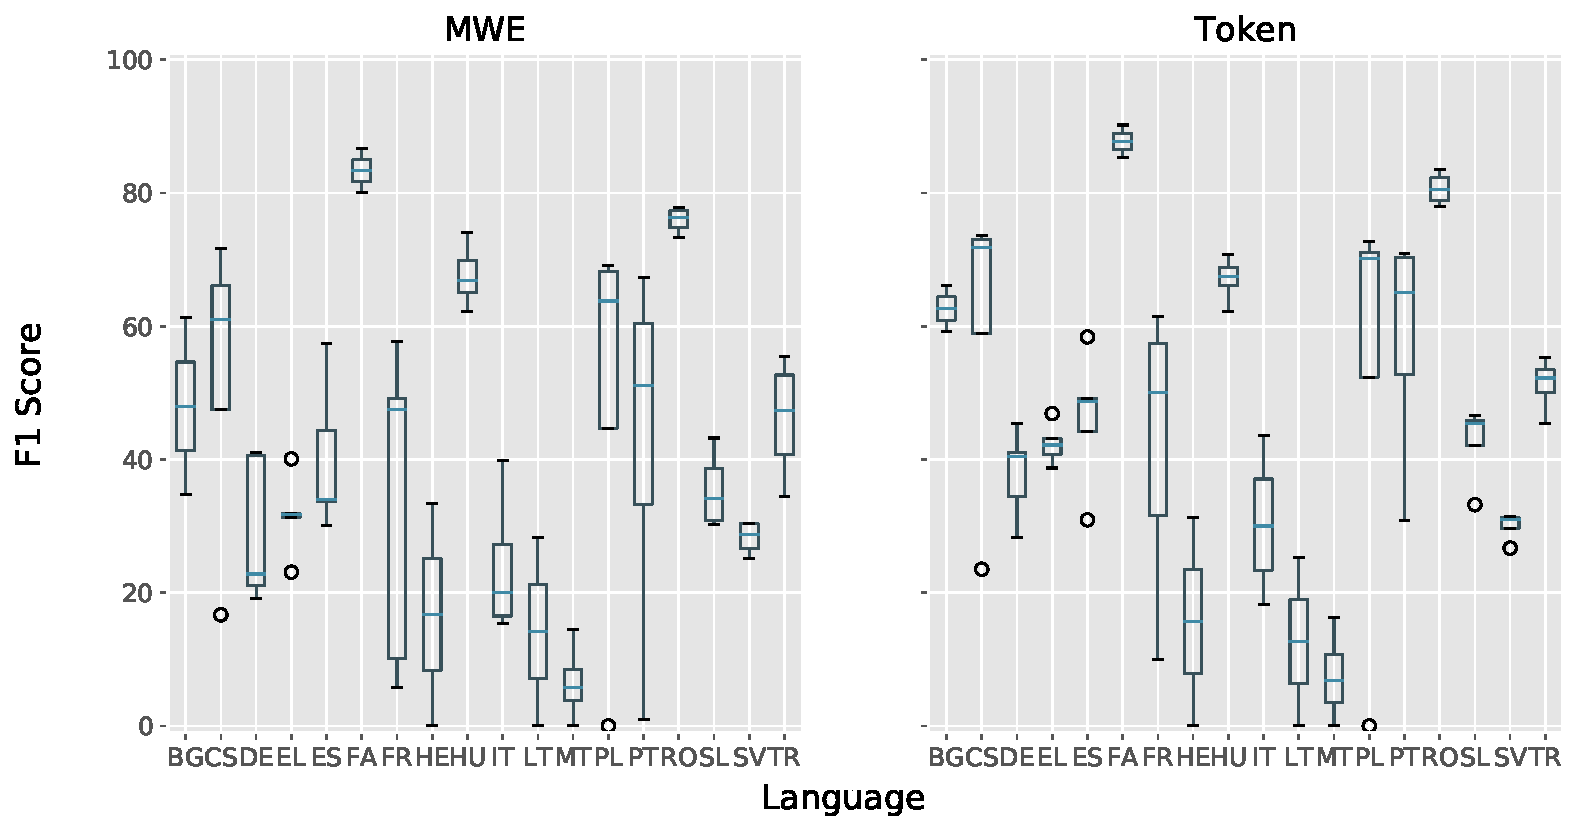
\includegraphics[scale=0.45]{figures/sys-f1-boxplots.pdf}
\caption{\label{fig:sys-f1-boxplots}Box plots summarising F1 scores achieved by all systems on each language, using the MWE-based and Token-based evaluation modalities}
\end{figure}

\subsection{\label{sec:corpus-overview}Corpora sizes, VMWE sparsity and frequency distributions}

We start by discussing the sizes of the training and test portions in each language corpus,\is{verbal multiword expression!sparsity}\is{PARSEME!corpus} depicted in \figref{fig:langcorp-sizes}. Sizes are measured in terms of the total number of sentences. Traditionally, corpora sizes are discussed in terms of number of words, rather than number of sentences. We use number of sentences instead for a variety of reasons: 1)~Each language corpus in the dataset consists of a collection of individual sentences. So the sentence is a natural unit to describe the dataset. 2)~A sentence is expected to have a single main verb. On average, we can expect to have a little more than one verb per sentence. However, we would like to know what this average is for the case of \emph{verbal} MWEs (VMWEs). That is, we would like to know how sparse VMWEs\is{verbal multiword expression!sparsity} are in a given language corpus, and what impact this sparsity may have. 3)~Measures such as the rate of VMWEs per $n$ tokens could also be used, but are less linguistically motivated. Finally, 4)~the training-to-test size ratios in terms of number of words are largely the same in this dataset as in terms of number of sentences. 

Notice that \ili{Romanian} and \ili{Czech} have by far the largest training sets, dwarfing corpora of all other languages. This seems to work in favour of these two languages as, on average, \ili{Romanian} ranked 2nd place in both evaluation modalities and \ili{Czech} ranked at 4th and 5th places in the MWE-based and Token-based modalities, respectively. \ili{Swedish} is the language with the smallest training set (only 200 sentences). The average F1 score of systems participating in \ili{Swedish} is around 30\% for both evaluation modalities. Indeed, the size of the training set is somewhat positively correlated with the average system evaluation scores for each language. The Pearson correlation coefficients for MWE-based and Token-based evaluations are 0.33 and 0.35, respectively.

The size of the test set relative to its corresponding training set varies widely across languages. The test-to-training proportions vary from 8\% to 60\% for most languages, except for \ili{Maltese} (79\%), \ili{Spanish} (85\%) and most notably, \ili{Swedish}, with a test set about 8 times larger than its training set (200 training sentences vs. 1600 test sentences), which makes the proportion of the training set almost invisible in \figref{fig:langcorp-sizes}. Although both \ili{Maltese} and \ili{Swedish} performed rather poorly (\ili{Maltese} actually ranked last), there is no clear pattern between the test-to-training proportion of a language corpus and the performance of systems. In fact, \ili{Spanish} ranked exactly in the middle at 9th place. These proportions were found to be mildly negatively correlated against MWE-based and Token-based evaluations: -0.20 and -0.23, respectively (Pearson correlation coefficients).

\begin{figure}
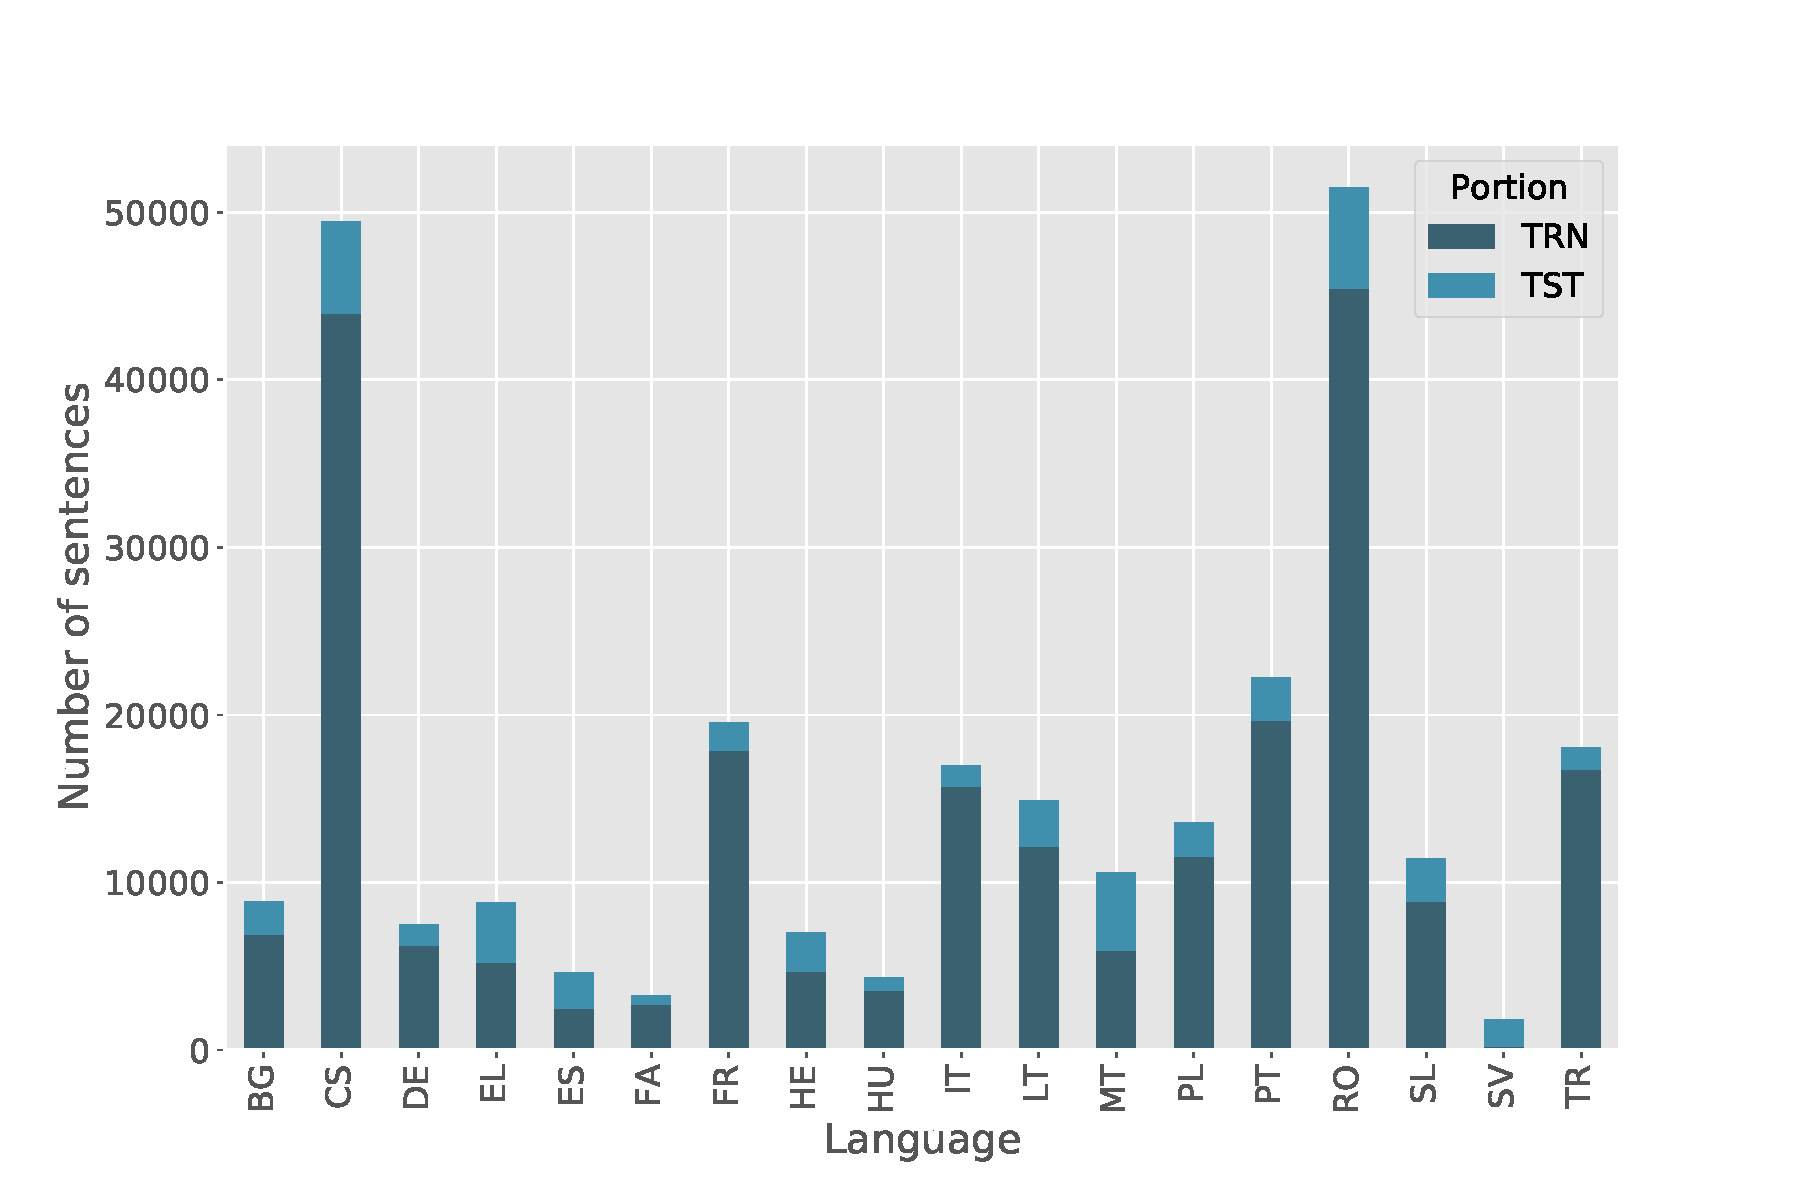
\includegraphics[scale=0.41]{figures/langcorpora-sizes-sents.pdf}
\caption{\label{fig:langcorp-sizes} Relative sizes (in sentences) of the training and test portions of each language corpus.}
\end{figure}

\begin{figure}
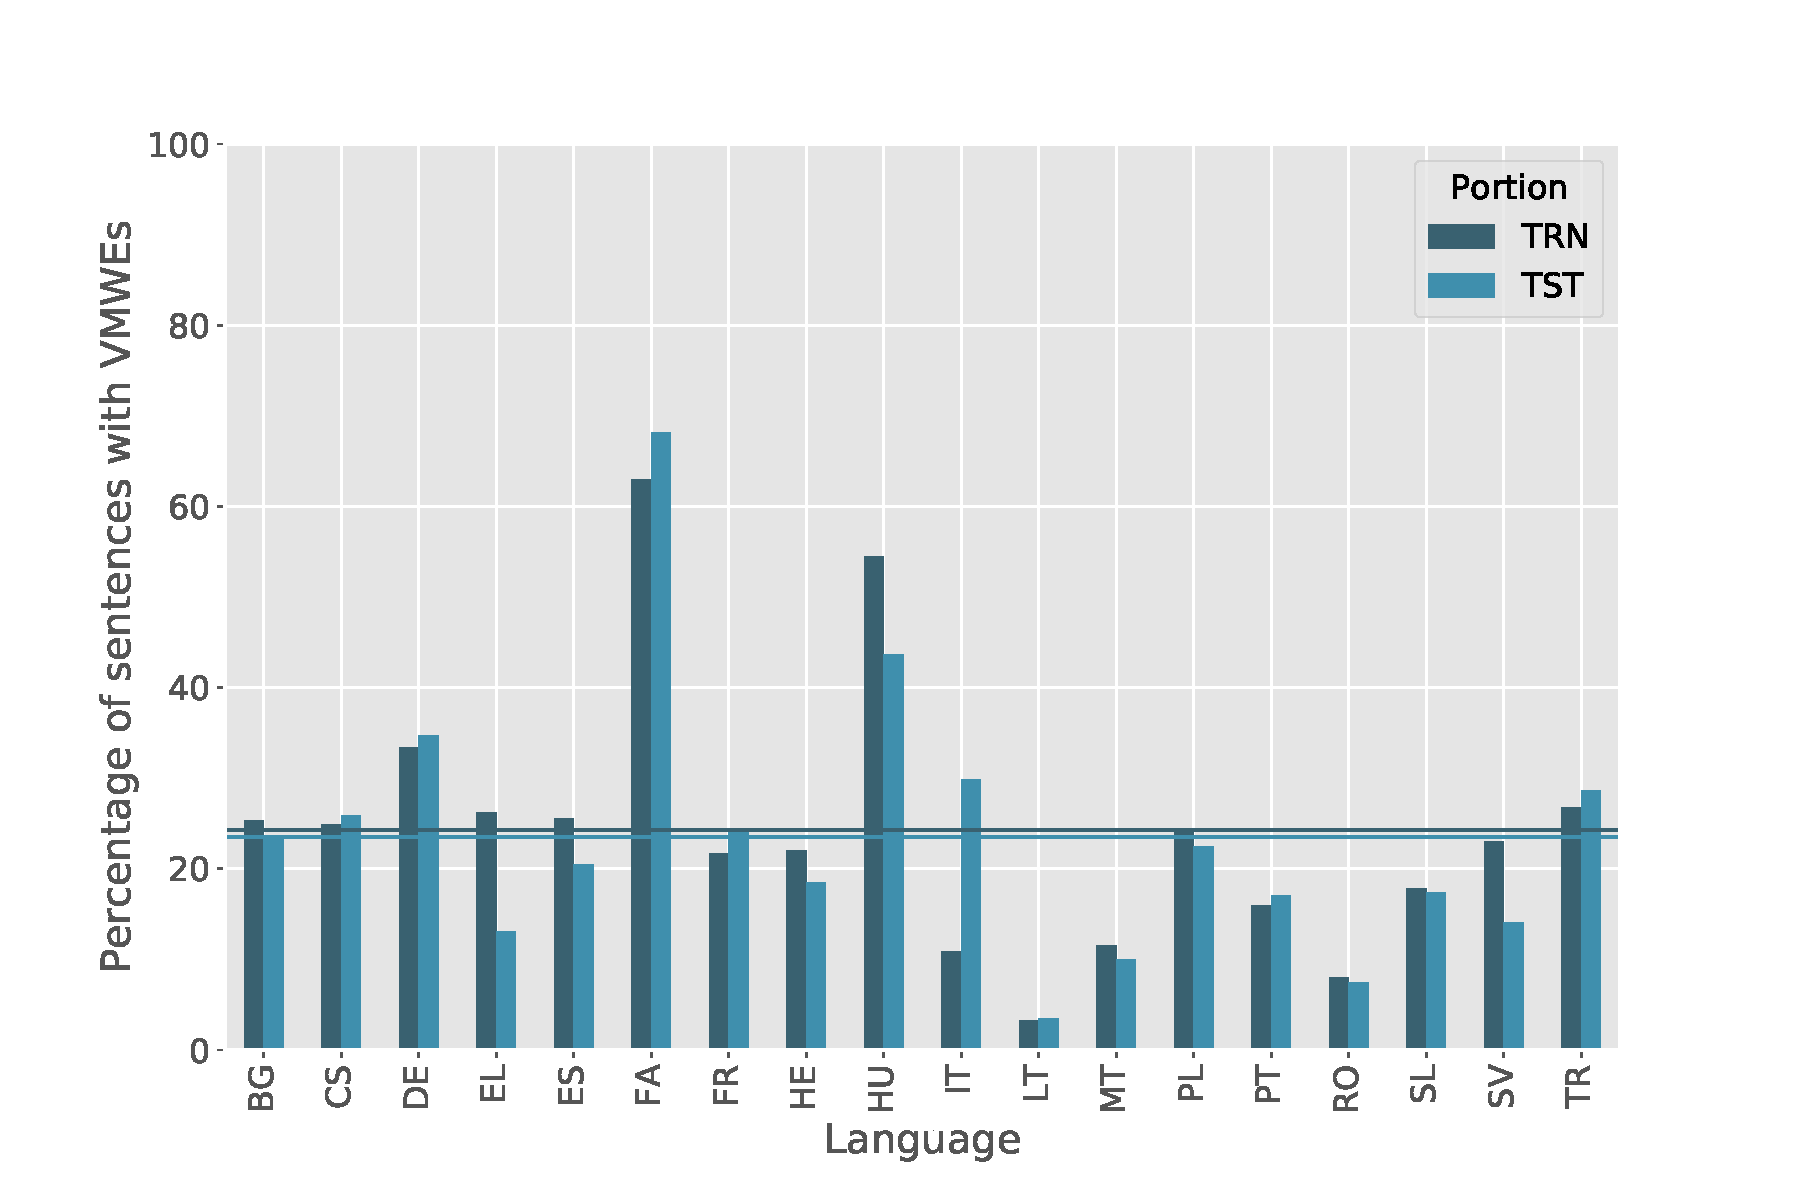
\includegraphics[scale=0.41]{figures/prop-sentswithmwes.pdf}
\caption{\label{fig:abs-props}VMWE Sparsity -- Percentage of sentences with VMWEs; horizontal lines depict average percentages across languages for training (TRN) and test (TST) sets, respectively.}
\end{figure}

\figref{fig:abs-props} shows how sparse VMWEs\is{verbal multiword expression!sparsity} are in the language corpora. VMWE sparsity\is{verbal multiword expression!sparsity} can be understood as the inverse of the proportion of sentences that have at least one VMWE. The figure shows the proportion of VMWEs within each set (training and test) using percentages. The graphs show that language corpora differ widely in their VWME sparsity. The overall proportion average (depicted by the two horizontal lines in the figure) is 24\% and 23\% for the training and test sets, respectively. Only \ili{Farsi} and \ili{Hungarian} are well above this average, and \ili{German} is slightly above. For most languages, the vast majority of sentences do not contain a single VMWE. Whilst sentences without VMWE examples are indeed needed by machine learning algorithms, too few examples could hinder learning processes due to class imbalance. Indeed, there is a strong positive correlation between the proportion of sentences with VMWEs and the average system evaluation scores: 0.58 Pearson correlation coefficient against MWE-based evaluation and 0.56 against Token-based evaluation. \ili{Lithuanian} and \ili{Maltese} are the two lowest scoring languages in both evaluation modalities (see \tabref{tbl:official-f1} and \figref{fig:sys-f1-boxplots}). They are two of the three languages with the highest VMWE sparsity. The third language is \ili{Romanian}, which turns out to be the second highest scoring language. \ili{Romanian} is, as previously mentioned, the language with the largest amount of training data. The \ili{Romanian} corpus' large volume seems to outweigh its high VMWE sparsity in systems' performance. 

Another feature which seems to help systems perform well in the \ili{Romanian} corpus is the \isi{frequency distribution} of its VMWEs, as shown in \figref{fig:matched-mwes}. This figure shows how many VMWE types occur at each VMWE frequency and how many of those VMWEs are successfully retrieved by the systems on the test portion of each language corpus. The grey bars on each chart show the total number of VMWE types occurring at each frequency inscribed on the $x$ axis. The coloured bars count the number of VMWE types at each frequency that were fully detected by each system. This figure shows that \ili{Romanian} VMWEs are \emph{well distributed}: whilst \ili{Romanian} hapax legomena (VMWEs occurring only once) dominate with 208 instances, there are many VMWEs with higher frequencies. The total number of VMWEs that occur more than once is 292, with frequencies up to 31 well represented. By contrast, 88 \ili{Lithuanian} VMWEs appear only once and the rest, 12 of them, just twice! For \ili{Maltese}, 82.57\% of its VMWEs are hapax legomena. The remaining 17.43\% have frequencies between 2 and 9. In short, VMWEs in the \ili{Lithuanian} and \ili{Maltese} corpora are not as well distributed by frequency as those in the \ili{Romanian} corpus. The less frequent a VMWE is, the less opportunities a system has to learn it. So if the majority of VMWEs in a corpus are of low frequency (as in \ili{Lithuanian} and \ili{Maltese}), it will be harder for a system to learn them, which will lead to potentially low performance scores for the system.

\begin{figure}
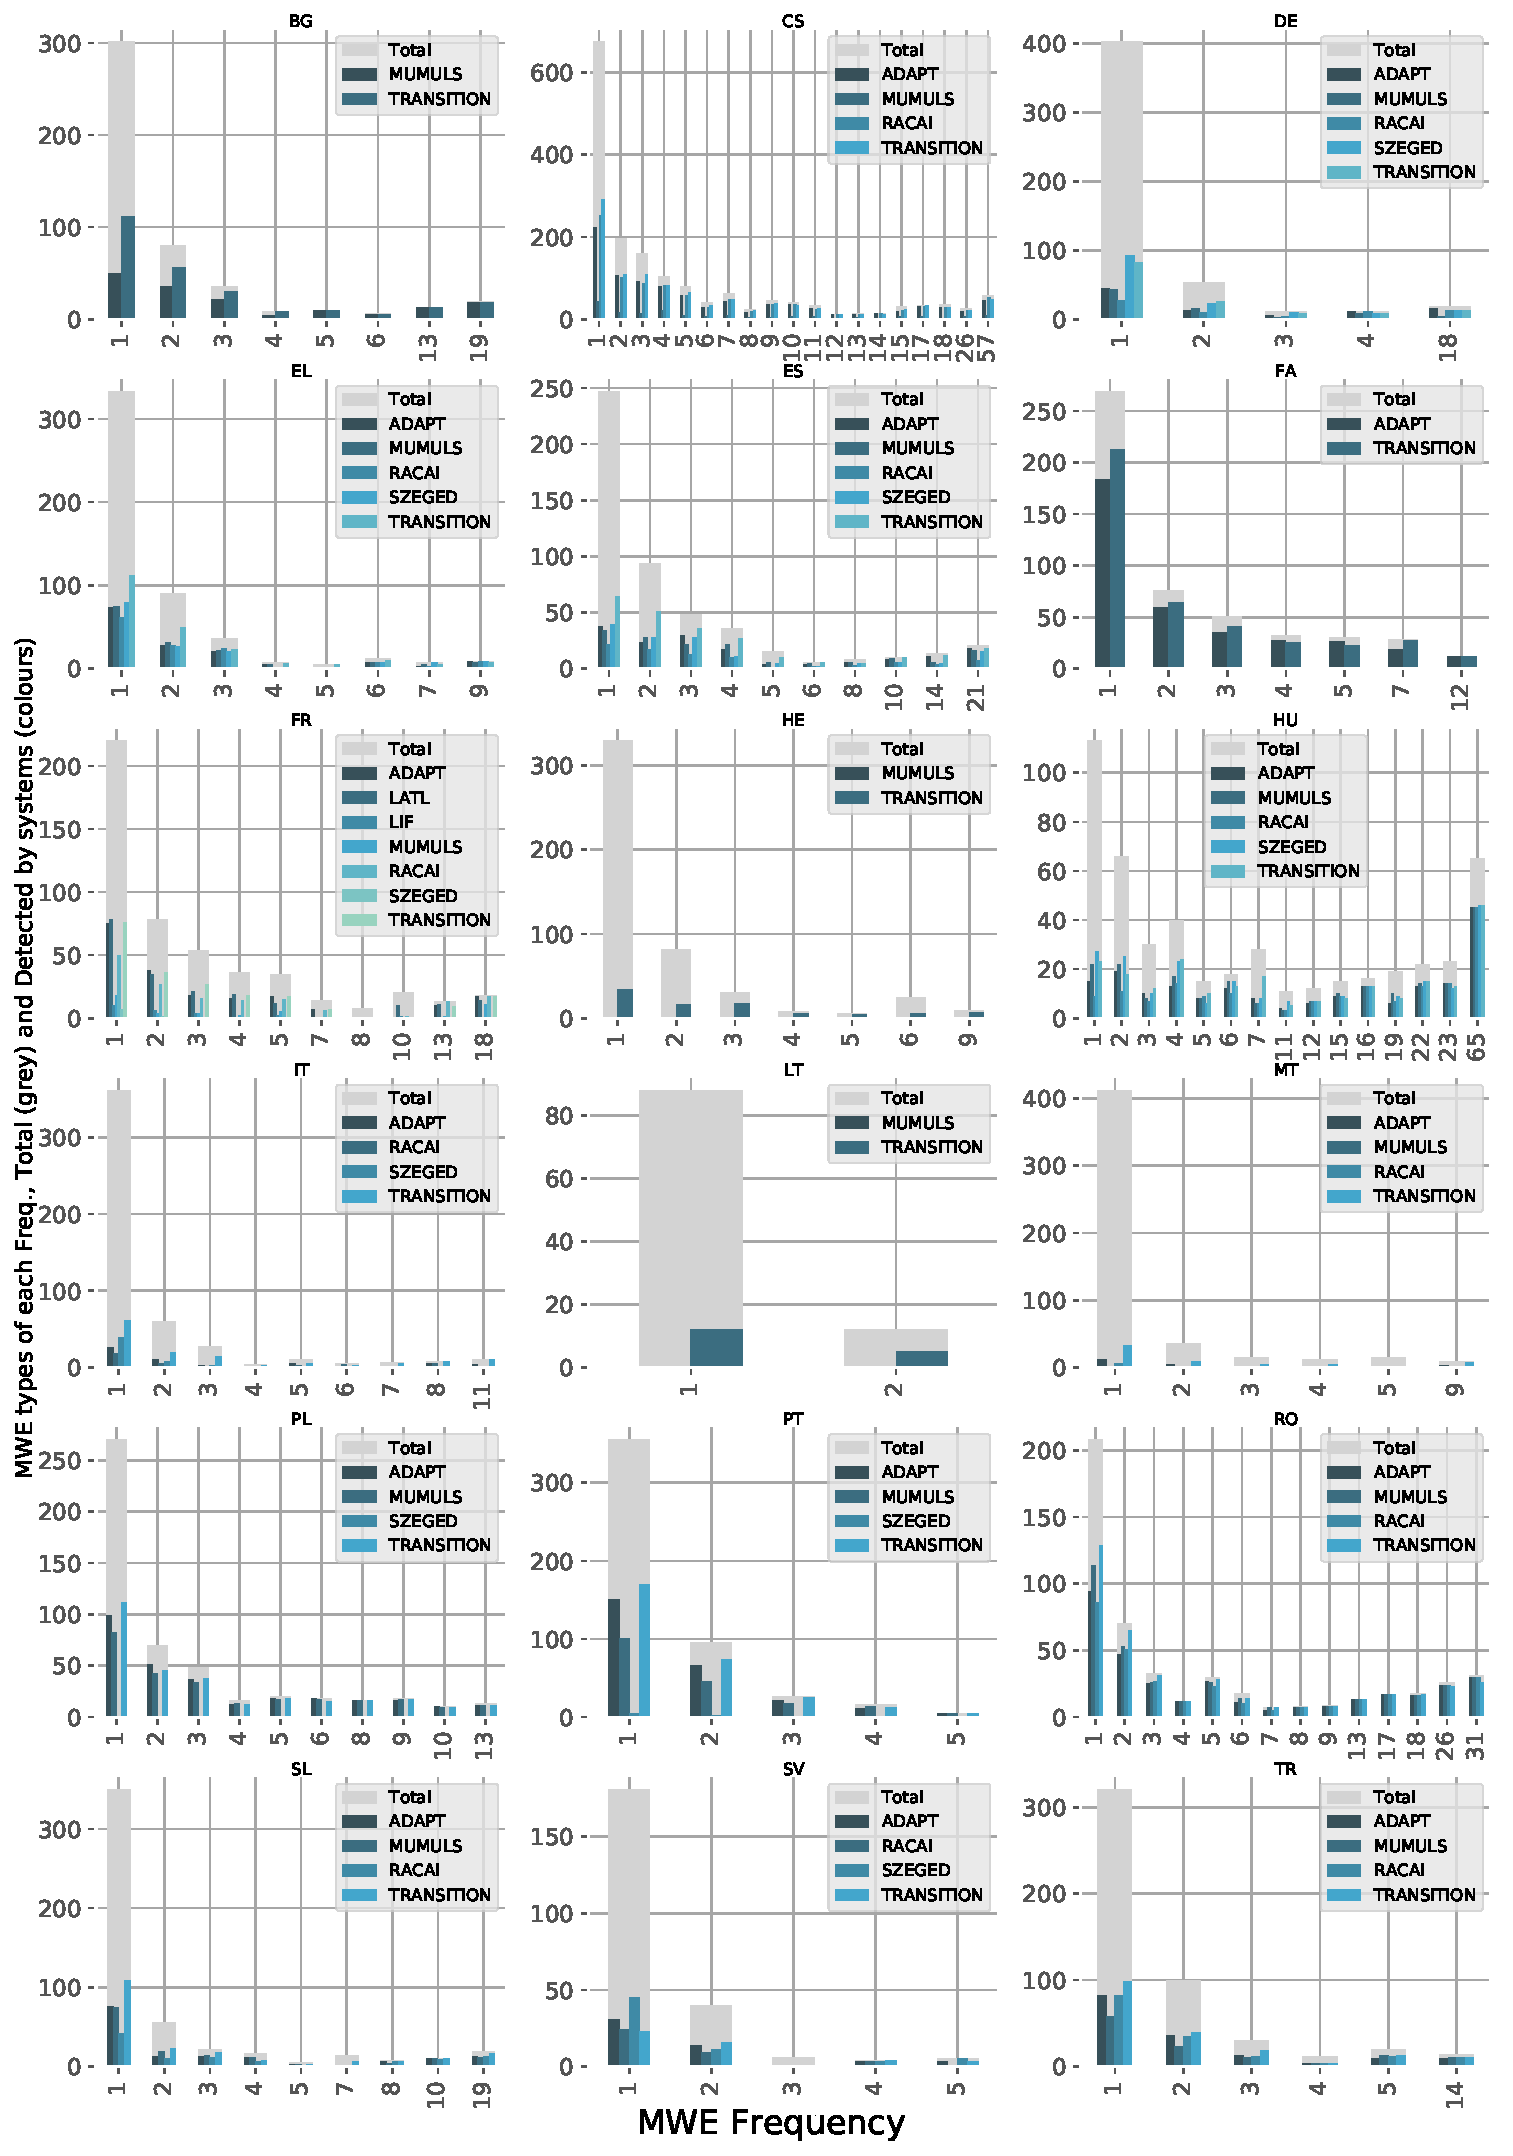
\includegraphics[scale=0.48]{figures/matched-mwes.pdf}
\caption{\label{fig:matched-mwes}Distribution of VMWEs of different frequencies on the test set (grey bars) and the proportion of such VMWEs detected by systems (coloured bars) based on full MWE-based detection.}
\end{figure}

As an aside, the grey bars in \figref{fig:matched-mwes} show, for most languages, that the majority of VMWEs are hapax legomena and that the number of VMWEs occurring more frequently decreases dramatically as their frequency increases. This is the hallmark of the Zipfian distribution, which is something to be expected with lexical phenomena \citep[pp.~22--6]{Manning}. This is not the usual way in which this distribution is traditionally plotted from data. However, it can be seen that most charts follow it approximately.

The issue of \emph{frequency distribution} is important. \ili{Hungarian} and \ili{Spanish} are modest in size in comparison with \ili{Lithuanian} and \ili{Maltese} (see \figref{fig:langcorp-sizes}), and yet the systems perform better in the former languages (especially in \ili{Hungarian}) than in the latter languages. \figref{fig:matched-mwes} reveals that both \ili{Hungarian} and \ili{Spanish} are well distributed by frequency. \ili{Hungarian}, despite having a smaller test set, is in fact even better distributed by frequency and has a lower VMWE sparsity (\figref{fig:abs-props}) than \ili{Spanish}.  It obtains a 67 average F1 score whereas \ili{Spanish} gets an F1 score average of 40--46, in both evaluation modalities (see \emph{avg}~column in \tabref{tbl:official-f1}).

From these observations, we can point out that language corpora with small amounts of training data, especially when combined with high VMWE sparsity\is{verbal multiword expression!sparsity} and a poor \isi{frequency distribution}, tend to obtain low scores in most systems. So increasing the size of training and test data is definitely a recommendation to follow. VMWE sparsity can be reduced by simply trying to balance out sentences with VMWEs against sentences without VMWEs. However, corpus designers should be cautious of doing this, as it could lead to a corpus that does not reflect the real distribution of VMWEs in the language and/or domain in question. Perhaps, it should be the task of system developers to design systems capable of coping with the natural VMWE imbalance/sparsity in a language corpus.\footnote{Systems could, for example, run a classifier to distinguish sentences that contain VMWEs from sentences that do not, and train/run their VMWE extractors only on sentences that do.} Improving the VMWE \isi{frequency distribution} in language corpora could also help systems. Ensuring that several examples of each VMWE type are included in the training data will be a challenge, however, due to the natural Zipfian tendency of a majority of VMWEs to appear only once in any given corpus. We propose offsetting this tendency by aiming to compile a corpus where the total frequency of VMWE types that occur \emph{frequently enough} outnumber the total frequency of VMWE types that occur \emph{less frequently}. That is, if $\theta$ is the minimum frequency a VMWE needs to have in order to be considered to have \emph{enough frequency},\footnote{$\theta$, a minimum desirable frequency, is a parameter to be set empirically, with $\theta=2$ a reasonable default value.} then we could ensure that the language corpus satisfies the condition:

\[
\sum_{v_{i}\in\{f(v_{j})\geq\theta\}}f(v_{i})>\sum_{v_{k}\in\{f(v_{j})<\theta\}}f(v_{k})
\]
where $f(v)$ is the frequency of VMWE $v$ in the corpus. Note that a corpus with a good VMWE \isi{frequency distribution} cannot be created by simply increasing the size of the corpus, but by better selecting sentences that are good examples of as many VMWEs as possible. 

\subsection{\label{sec:shared}VMWEs shared between the training and test sets}

\citet{maldonado2017} noticed that the proportion of VMWEs shared between the training set and the test set of a language corpus is strongly positively correlated with the performance scores achieved by participating systems on that language test set (see also \citealtv{Savarytv} §6.3). The most likely explanation is that when evaluated on the test set, machine learning systems would tend to perform better on VMWE examples they encountered in the training set (i.e. exact VMWEs that systems have already \emph{seen} during training)\is{verbal multiword expression!seen} than on VMWE examples that systems encounter for the first time in testing. The higher the proportion of shared/seen VMWEs is in one language, the higher a machine learning system can be expected to perform on that language. \figref{fig:f1-vs-ps-all} depicts this relationship by plotting the score achieved by each system on each language against the proportion of shared/seen VMWEs in that language. The languages on the $x$ axis are sorted and labelled by this proportion. Notice the near-linear relationship between this proportion and the system scores.

\begin{figure}
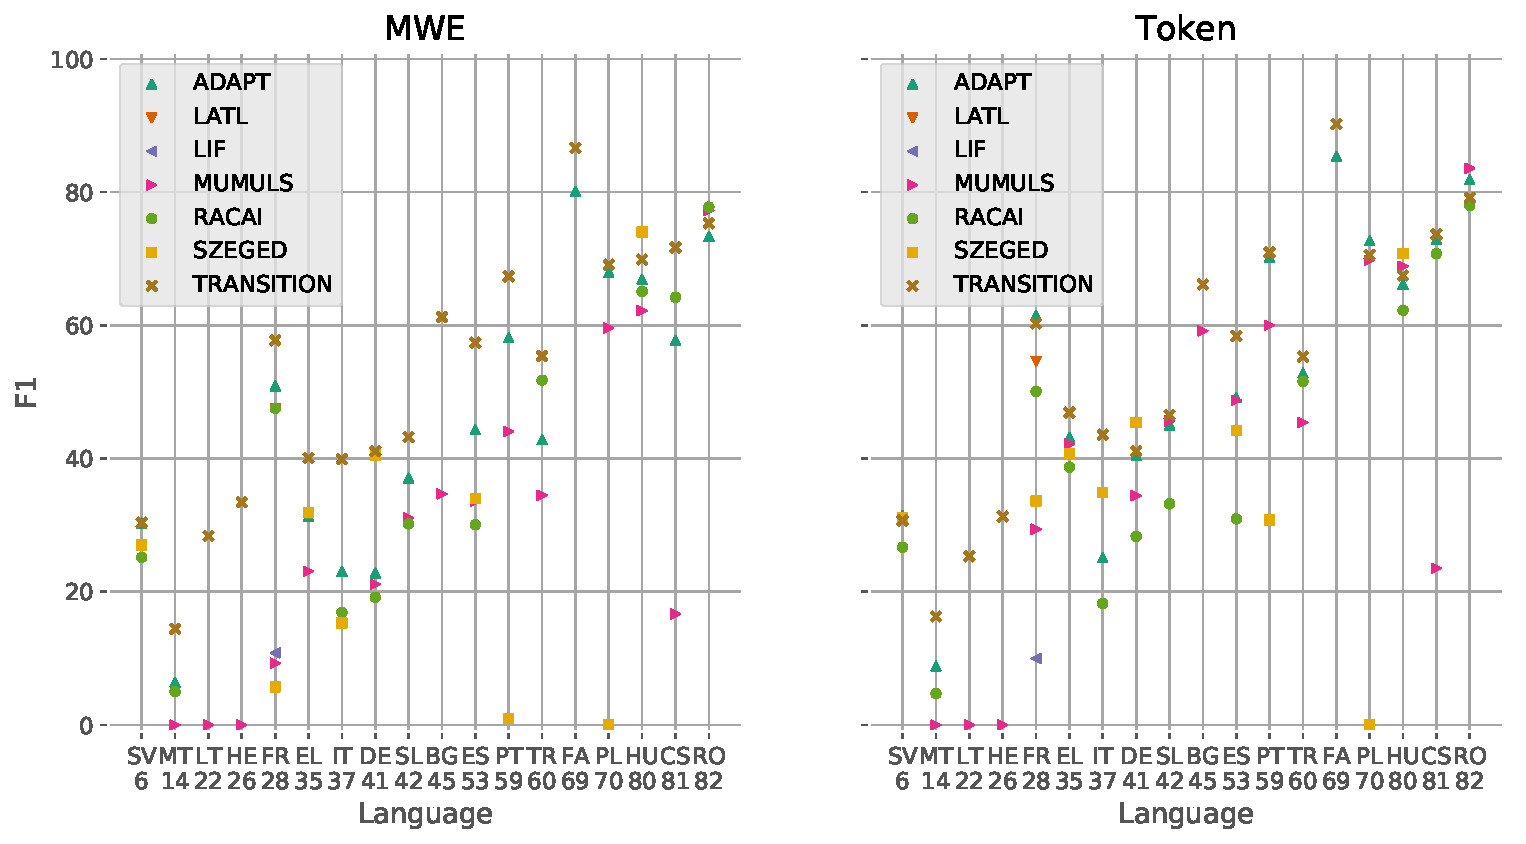
\includegraphics[scale=0.45]{figures/sys-f1-vs-ps-allvmwes.pdf}
\caption{\label{fig:f1-vs-ps-all}System evaluation scores (MWE-based, left; Token-based, right) for each language against the proportion (percentage) of test VMWEs seen during training}
\end{figure}

\begin{figure}
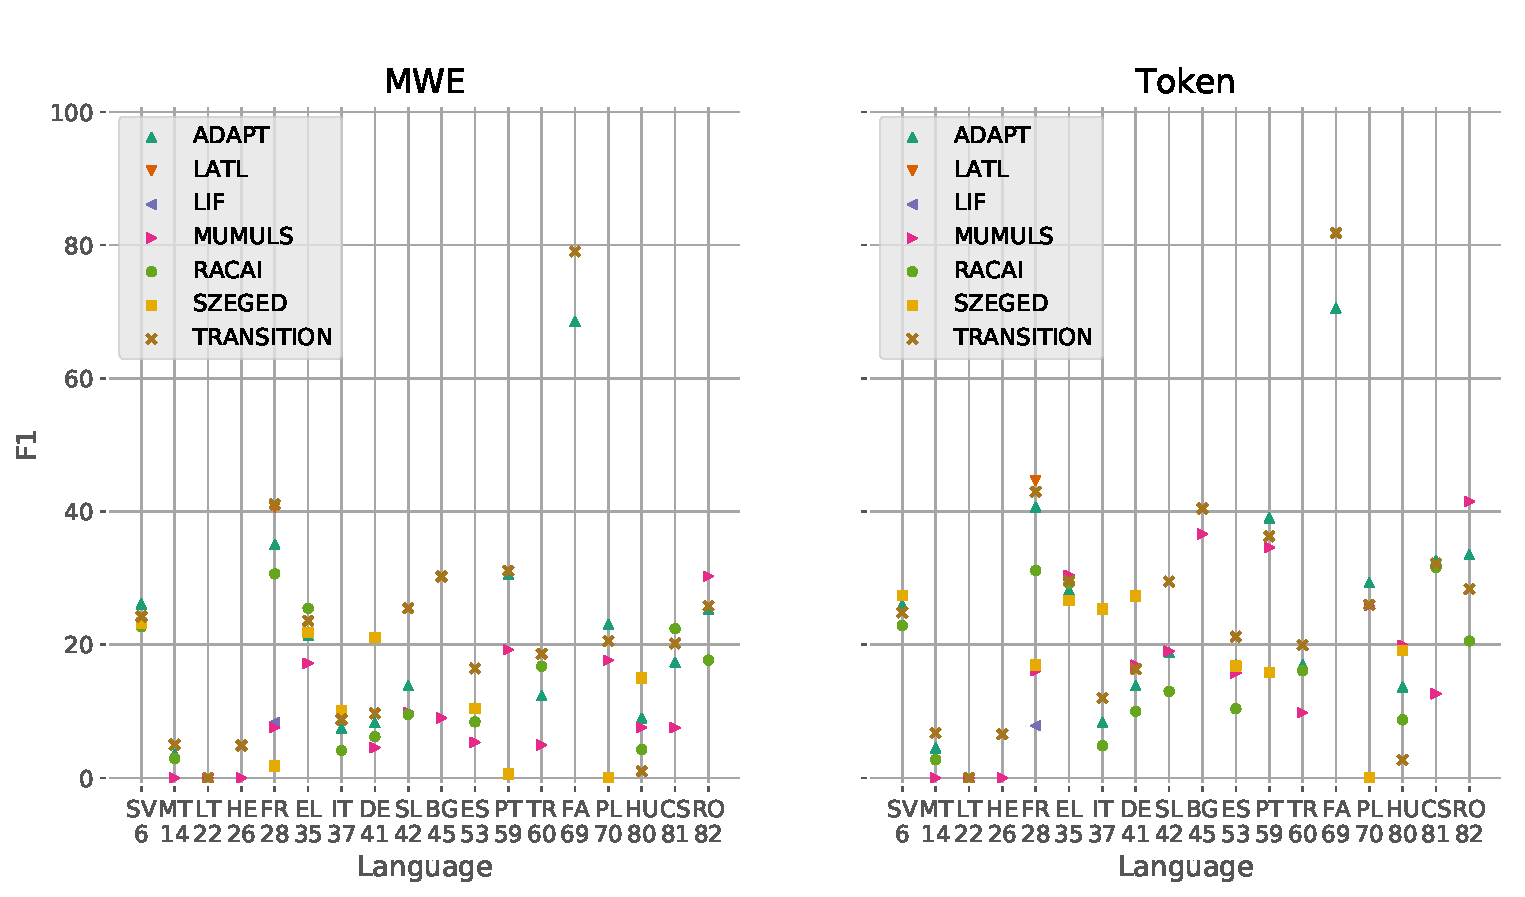
\includegraphics[scale=0.45]{figures/sys-f1-vs-ps-newvmwes.pdf}
\caption{\label{fig:f1-vs-ps-new}System evaluation scores (MWE-based, left; Token-based, right) on non-shared/unseen VMWEs only}
\end{figure}

It is of interest to evaluate systems on non-shared/unseen\is{verbal multiword expression!unseen} VMWEs only. This can be done by using the official systems' outputs, which were kindly provided to us by the shared task organisers. In order to evaluate unseen VMWEs only, the labels for seen VMWEs in the systems' outputs and the gold standards were cleared (i.e. changed to the underscore `\_' flag) so that they would be ignored by the official evaluation scripts. \figref{fig:f1-vs-ps-new} shows the systems' performance scores when evaluated in this manner on unseen VMWEs only. Notice that the $x$ axis was kept from \figref{fig:f1-vs-ps-all} to enable an easy visual comparison between both figures.

The first thing to notice is that all systems' scores go down dramatically for all languages. Notice however that for \ili{Farsi}, the TRANSITION and ADAPT scores do not fall as dramatically as in the other languages. At first glance, this can be associated with the density of annotated instances of VMWEs in the \ili{Farsi} corpus, i.e., \ili{Farsi} has the lowest VMWE sparsity in the dataset (as discussed in \sectref{sec:corpus-overview}). On the other hand, the second least VMWE-sparse language, \ili{Hungarian}, did not fare nearly as well in this unseen VMWE evaluation. Taking a closer look at \ili{Farsi} VMWEs, we observe that they show a higher level of \emph{collostructional regularity}\footnote{Degree to which words tend to form (appear with) grammatical constructions \citep{collostructional}.} compared to VMWEs in other languages. We observe that 86\% of \ili{Farsi} VMWEs are of length 2 and the last token in all \ili{Farsi} VMWEs is always a verbs, while this is not the case for other languages such as \ili{Hungarian}. In addition, verbs constitute a relatively small vocabulary in \ili{Farsi} and as a consequence, the same set of verbs are used repeatedly in various VMWEs. For example, the 2,707 annotated VMWEs in the \ili{Farsi} training set end with verbs of 46 different lemmas, and the 500 annotated instances in the test set end with 34 lemmas. Among these 34 different lemmas, only 4 do not appear in the training set. Last but not least, most of these verb lemmas are strong indicators of the presence of VMWEs, too. The overall occurrences of these lemmas in the \ili{Farsi} corpus is 6,969, from which 3,207 are part of a VMWE, i.e., nearly half of them (46\%). More precisely, 16 of these lemmas (with 29 occurrences) appear only as constituents of VMWEs; most importantly, for the most frequent lemma in VMWEs (the past and present forms of the infinitive {\RL{\Parsifont کردن}} /kærdæn/ \lit{to make/to do}, a light verb, which appears as the verb in 1,096 VMWEs) this proportion is 97\% (i.e., out of 1,128 occurrences of this verb, only 32 do not surface as VMWE). To this, we can add observations concerning syntactic patterns in which VMWEs are used, e.g., the light verb {\RL{\Parsifont کردن}} /kærdæn/ usually forms a transitive VMWE in which the non-verbal component of the VMWEs appear right after the adposition  {\RL{\Parsifont را}} /ra/ (i.e., which signals the presence of the syntactic object).  We maintain that these exemplified regularities can justify the obtained results over the \ili{Farsi} corpus.  
%\textcolor{red}{
%This being said, however, we would like to emphasise that this observation does not hold for all VMWEs. For instance, in nearly 10\% of the annotated VMWEs (316 instances) the verbs are /æst/ and /bud/, which are mainly and frequently used as copulas (equivalent to \emph{to be} in \ili{English}) -- with 2,297 occurrences in the FA corpus.  --- alfredo we can remove this [alfredo: I'm OK with removing this]}

%Train size of annotated data: 2707
%Number of light verb forms in test 69
%Number of light verb lemmas in test 34
%----
%Number of light verb forms in train 117
%Number of light verb lemmas in train 46
%--
%Light verb forms only in test 29
%Light verb lemmas only in test 6
%[افتاده, بر, نمود, بُرد, ياب, آويخت]


%\textcolor{red}{This is perhaps due to the fact that \ili{Farsi} has the lowest VMWE \isi{sparsity} in the dataset (as discussed in Section~\ref{sec:corpus-overview})} \textcolor{blue}{and special characteristics of Farsi} . 

 In general, however, it is fair to expect that systems will tend to perform worse on VMWEs they did not see in training.  
 %\textcolor{red}{In the case of \ili{Farsi} vs \ili{Hungarian}, it could well be that \ili{Farsi} VMWEs are just easier to identify. That is, there is a linguistic feature in \ili{Farsi} that works on the systems' favour. -- [alfredo] Behrang: I think we can remove this sentence, as you already talked at length about \ili{Farsi} vs \ili{Hungarian}. Do you agree?}

%% EXPLAIN WHAT'S GOING ON WITH SWEDISH? IT DOESN'T GO DOWN VERY MUCH BECAUSE IT'S MOSTLY MADE OF NEW VMWEs ANYWAY.

\subsection{Discontinuous VMWEs and embedded/overlapped VMWEs}
Two innovations in the PARSEME shared task\is{PARSEME!shared task} were discontinuous VMWEs and embedded or overlapped VMWEs (see \citealtv{Savarytv} §6.3).\is{verbal multiword expression!discontinuity}\is{verbal multiword expression!nesting}\is{verbal multiword expression!overlapping}


\figref{fig:cont} shows that for most languages, the majority of VMWEs are continuous. For \ili{Czech} and \ili{Turkish}, there is about a 50--50 proportion between continuous and discontinuous VMWEs. For many other languages, the proportion of discontinuous VMWEs is considerable (\ili{German}, \ili{Greek}, \ili{French}, \ili{Polish}, Portuguese\il{Portuguese!Brazilian}, \ili{Romanian}, Slovenian). There is therefore a clear advantage in designing systems capable of detecting discontinuous VMWEs.

\begin{figure}
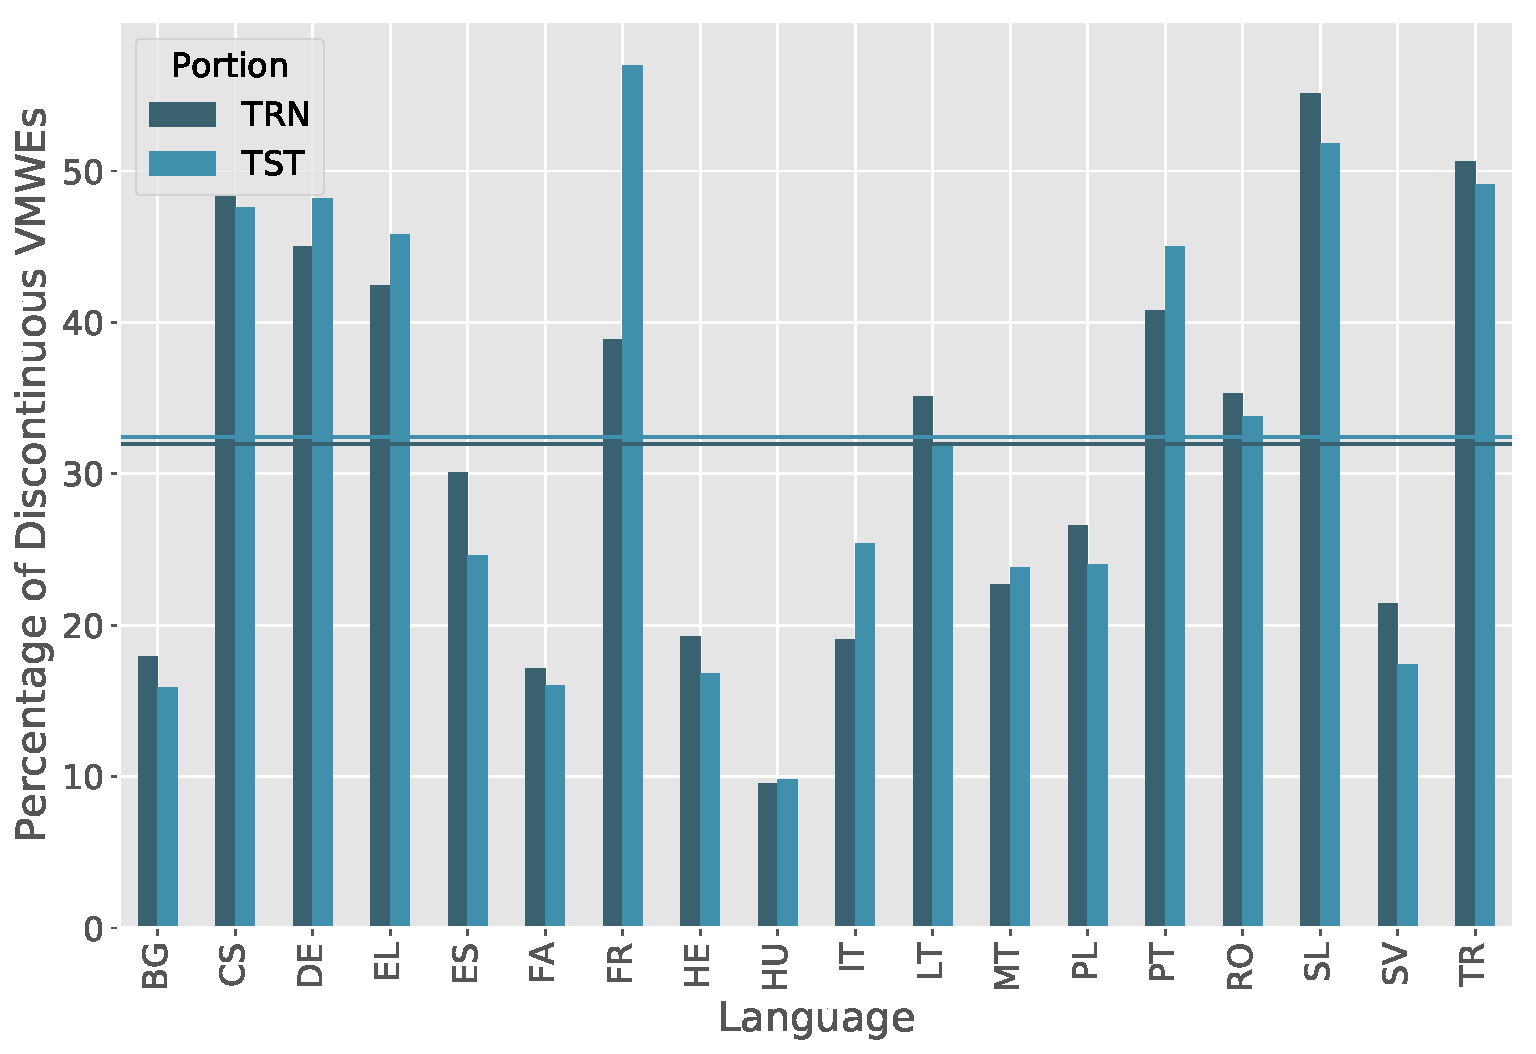
\includegraphics[scale=0.45]{figures/noncont-perc.pdf}
\caption{\label{fig:cont}Percentage of discontinuous VMWEs across language corpora.}
\end{figure}

\begin{figure}
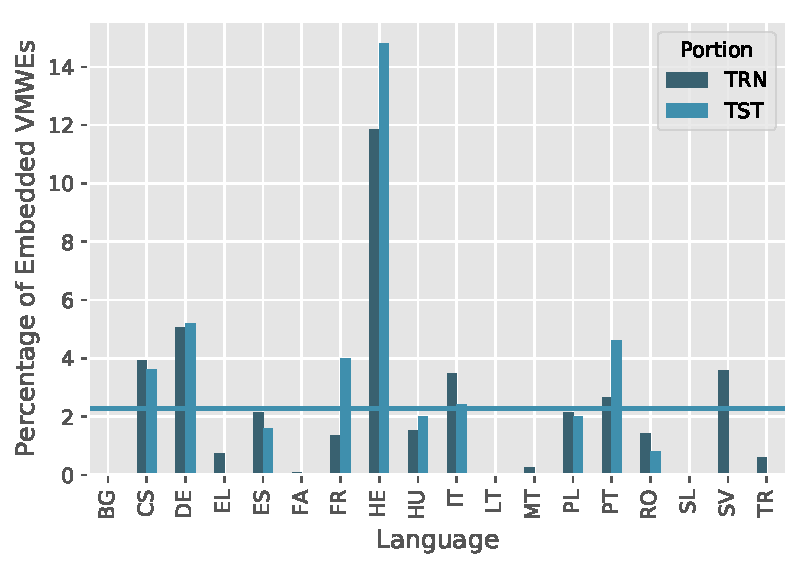
\includegraphics[scale=0.45]{figures/emb-perc.pdf}
\caption{\label{fig:embedded}Proportion of Embedded/Overlapped VMWEs across language corpora.}
\end{figure}

The proportion of embedded/overlapped VMWEs, shown in \figref{fig:embedded}, is very low across languages, with an average of around 2.3\% in both training and test portions. \ili{Hebrew} is the language with the highest rate of embedded VMWEs at only 12--14.5\%.  Some languages do not even register a single embedded VMWE. Because of these low numbers, a system not designed to deal with embedded VMWEs will not be severely penalised. We therefore do not consider embedded VMWEs to be a difficulty factor in this dataset, with the exception of \ili{Hebrew}.

\subsection{Relative training-test corpus heterogeneity}

The evaluation paradigm followed in the PARSEME shared task\is{PARSEME!shared task} dictates that systems must be evaluated on a strictly unseen\is{verbal multiword expression!unseen} test set, guaranteeing fairness to all participating system developers. However, a valid expectation is that the data that systems will be tested on should be roughly of the same kind as the data they were trained on. The training and test portions of a language corpus should be fairly homogeneous.\is{corpus!heterogeneity}\is{corpus!homogeneity}

\citet{Kilgarriff1998} introduced a statistical metric to estimate the similarity of two corpora of similar size by computing the $\chi^{2}$ score of the $n$ most frequent words in the corpora. The lower this score, the less variability between the corpora and thus the more similar they are. They also adapted this similarity score to measure the homogeneity of a single corpus by computing $\chi^{2}$ scores on pairs of similarly sized partitions of the corpus and averaging the individual $\chi^{2}$ scores. The lower this averaged score is, the more homogeneous the corpus is deemed to be. Here, we adapt this homogeneity score in order to estimate the homogeneity between the training and test sets of a language corpus. This is done by computing similarity scores of training set partitions against similarly-sized test set partitions and averaging them together to obtain a single cross-set homogeneity score. The higher this score is, the more heterogeneous the training and test sets are. In order to allow comparisons across languages, this cross-set homogeneity score is normalised by dividing it by the average of the within-training set and within-test set homogeneity scores, calculated from the training and test sets separately. We call the result of this division, the \emph{heterogeneity ratio of a language corpus}. \tabref{tbl:homogeneity} sorts the languages by their heterogeneity ratio. The detailed algorithm used is listed in Algorithm~\ref{alg:heterogeneity-ratio}.

\begin{table}
\caption{\label{tbl:homogeneity}Heterogeneity ratios between training and test sets}

{\scriptsize{}}%
\setlength\tabcolsep{3.0pt} % col separation
\renewcommand{\arraystretch}{0.65} % row separation
\begin{tabular}{cccccccccccccccccc}
\lsptoprule 
{\scriptsize{}FR} & {\scriptsize{}TR} & {\scriptsize{}IT} & {\scriptsize{}PT} & {\scriptsize{}RO} & {\scriptsize{}CS} & {\scriptsize{}PL} & {\scriptsize{}HU} & {\scriptsize{}LT} & {\scriptsize{}DE} & {\scriptsize{}FA} & {\scriptsize{}BG} & {\scriptsize{}SL} & {\scriptsize{}ES} & {\scriptsize{}SV} & {\scriptsize{}HE} & {\scriptsize{}EL} & {\scriptsize{}MT}\tabularnewline
\midrule
{\scriptsize{}4.31} & {\scriptsize{}2.89} & {\scriptsize{}2.53} & {\scriptsize{}2.03} & {\scriptsize{}2.03} & {\scriptsize{}1.92} & {\scriptsize{}1.77} & {\scriptsize{}1.73} & {\scriptsize{}1.62} & {\scriptsize{}1.59} & {\scriptsize{}1.56} & {\scriptsize{}1.51} & {\scriptsize{}1.39} & {\scriptsize{}1.28} & {\scriptsize{}1.25} & {\scriptsize{}1.18} & {\scriptsize{}1.15} & {\scriptsize{}1.03}\tabularnewline
\lspbottomrule
\end{tabular}

\end{table}

\begin{algorithm}
\algrenewcomment[1]{$\:\:\:\:\:\:\:\blacktriangleright$ #1} % comments at the start of line, not at the end.
\caption{\label{alg:heterogeneity-ratio}Computing a language heterogeneity ratio}
{\fontsize{9}{9}\selectfont
\begin{algorithmic}[1]
\State $R \gets$ number of repetitions
\State $n \gets$ number of words in a partition
\State $hr\_sum \gets 0$
\State $r \gets 0$
\While{$r < R$}
    \State $trn \gets $ partition\_set($n$, shuffle\_sentences(training\_set))
    \State $tst \gets $ partition\_set($n$, shuffle\_sentences(test\_set))
    
    \\ \\
    \Comment{Cross homogeneity:}
    \State $s \gets 0$
    \State $c \gets 0$
    \For{$i=1$ to $|trn|$}
        \For{$j=1$ to $|tst|$}
            \State $s \gets s + $ corpus\_similarity($partition_i$, $partition_j$)
            \State $c \gets c + 1$
        \EndFor
    \EndFor
    \State $cross \gets s / c$

    \\ \\
    \Comment{Within-training homogeneity:}
    \State $s \gets 0$
    \State $c \gets 0$
    \For{$i=1$ to $|trn|$}
        \For{$j=i+1$ to $|trn|$}
            \State $s \gets s + $ corpus\_similarity($partition_i$, $partition_j$)
            \State $c \gets c + 1$
        \EndFor
    \EndFor
    \State $within\_trn \gets s / c$
    
    \\ \\
    \Comment{Within-test homogeneity:}
    \State $s \gets 0$
    \State $c \gets 0$
    \For{$i=1$ to $|tst|$}
        \For{$j=1+1$ to $|tst|$}
            \State $s \gets s + $ corpus\_similarity($partition_i$, $partition_j$)
            \State $c \gets c + 1$
        \EndFor
    \EndFor
    \State $within\_tst \gets s / c$
    
    \\ \\
    \Comment{Heterogeneity ratio:}
    \State $hr \gets cross / ((within\_trn + within\_tst)/2)$
    \State $hr\_sum \gets hr\_sum + hr$
    
    \\
    \State $r \gets r + 1$
\EndWhile

\State \textbf{return} $hr\_sum / R$
\end{algorithmic}
}
\end{algorithm}

\ili{French} comes out on top. Its heterogeneity ratio of 4.31 can be interpreted as the number of times that the training-test sets are more heterogeneous than the training and test sets on their own. This suggests that the \ili{French} test was not derived from the same sources as the training set, or at least not in the same proportions.

\ili{French} is followed by \ili{Turkish}, \ili{Italian}, Portuguese\il{Portuguese!Brazilian} and \ili{Romanian}, with ratios around 2. The rest of the languages are closer to 1, reflecting a more balanced/homogeneous partitioning between the training and the test corpora. Notice however that systems participating in \ili{French}, \ili{Turkish}, \ili{Italian}, Portuguese\il{Portuguese!Brazilian} and \ili{Romanian} did relatively well despite their heterogeneity. Nonetheless, adopting a similar corpus selection and balancing policy across languages, like mixing the corpora before splitting them into training and test portions in comparable proportions, could be a way to put all languages on a similar footing.


\begin{comment}
Points to cover:
* New vs "seen" VMWEs - concept and method of detecting them
* Graph comparing systems and baselines performance on \isi{shared task} against proportion of "seen" VMWEs (like the one in my poster)
* Evaluation on new VMWEs only: graph comparing systems and baselines 
* Discussion/Analysis of results - which approaches seem to be better at detecting new VMWEs? 
\end{comment}

\section{\label{sec:systems}Participating systems and baselines}

\begin{comment}
Points to cover (re-organised as per Behrang's feeback):
* An overview of the approaches used in participating systems
* Participating systems results
* Baselines description
* Graph comparing systems and baselines performance on \isi{shared task}
\end{comment}

This section focuses on the actual systems in the competition and introduces two baseline systems: (i) a dictionary lookup-based system that attempts to match known VMWEs against the test set, (ii) a system that flags every verb in the test set as a VMWE.

\subsection{Overview of participating systems}

Seven systems participated in the PARSEME shared task\is{PARSEME!shared task}\is{verbal multiword expression!identification}. Their performance was presented and discussed in \sectref{sec:dataset}, although not individually. The techniques employed by the different systems can be summarised as follows:

\begin{itemize}
    \item ADAPT \citep{maldonado2017} uses a Conditional Random Fields (CRF) sequence labelling approach to identify the tokens of VMWEs. The features that helped most were dependency-based: the token's head, dependency relation with the head and the head's part of speech (POS) tag, along with standard bigram and trigram features commonly used in named-entity recognisers. The ADAPT system did not attempt to classify VMWEs by category. An extended version of this system is described in \citetv{Moreautv}.
    \item RACAI \citep{borocs2017} also employs a CRF sequence labelling approach using lemma and POS tag features. However, this system conducts the VMWE identification task in two steps: head labelling (identifying the verb) and tail labelling (identifying the words linked to the head). The RACAI system does attempt to classify the VMWEs by their category. 
    \item MUMULS \citep{W17-1707} also models the VMWE identification problem as a sequence labelling task, but using a recurrent neural network via the TensorFlow package. As input features, they build embeddings of 100 dimensions from the concatenation of a token's surface form, lemma and POS tag. 
    \item TRANSITION \citep{W17-1717} is a greedy transition-based system of the kind typically used in parsing. This system does not have a syntax prediction module, however, and focuses on the lexical analysis phase of the parsing mechanism. An extended version of this system is described in \citetv{AlSaiedtv}.
    \item LIF \citep{MWEWorkshop} also employs a probabilistic transition-based technique. The team focused on \ili{French} light-verb constructions. 
    \item SZEGED \citep{Simko2017} trains a dependency parser on a modified training set in which the dependency relation label of tokens belonging to a VMWE were relabelled with the corresponding VMWE category label. \citetv{Simkotv} describes an extended version of this system.
    \item LATL \citep{W17-1706} uses a rule-based constituent parser that prioritises parsing alternatives of known collocations, and uses its parsing features to detect known collocations even if they are in a different word order or if they are discontinuous.
\end{itemize}

Not all systems participated in all languages. \ili{French} was the language covered by most systems. The languages least covered were \ili{Bulgarian}, \ili{Hebrew}, \ili{Lithuanian} (covered only by MUMULS and TRANSITION) and \ili{Farsi} (covered by ADAPT and TRANSITION). Since only raw surface tokens and no syntactic dependency information or POS tags were provided for \ili{Bulgarian}, \ili{Hebrew} and \ili{Lithuanian}, most system developers decided not to cover them. The systems that covered most languages were TRANSITION (all 18 languages), ADAPT (15), MUMULS (15), RACAI (12) and SZEGED (9). LATL and LIF focused on \ili{French} only. 

In Token-based evaluation, ADAPT ranked first on two languages (\ili{French} and \ili{Polish}), while MUMULS and SZEGED ranked first on \ili{Romanian} and \ili{Hungarian}, respectively. In MWE-based evaluation, TRANSITION beat all systems in all languages, except \ili{Hungarian} (won by SZEGED) and \ili{Romanian} (won by RACAI and very closely followed by MUMULS).

The ADAPT and the RACAI systems are clearly related, as are the TRANSITION and the LIF systems. These four systems, along with the MUMULS system, are all probabilistic sequence labelling methods, although quite different in their implementation details. It is interesting to see that, on average (see bottom row in \tabref{tbl:official-f1}), ADAPT and TRANSITION performed very similarly in the Token-based evaluation, while MUMULS and RACAI also performed very similarly in the same average evaluation. 

%% DIFFERENCES BETWEEN ALL AND NEW

%% PERFORMANCE PER CATEGORY

\subsection{\label{sec:baselines}Baseline systems}

This section proposes two types of baseline systems that put into perspective the participating systems' performance. One such baseline system is a simple dictionary lookup, which collects all VMWEs encountered during training and simply attempts to match collected VMWEs in the test set. The other is a baseline system which flags every verb as a VMWE. More details on these two baselines and their results are described in what follows. 

\paragraph*{Dictionary lookup baseline}

The implemented system is very simplistic: it attempts to match VMWE lemmas from the training file in the test file sequentially.\is{dictionary lookup baseline} If lemmas are not available, then the token's surface form is used. Discontinuous VMWEs\is{verbal multiword expression!discontinuity} are matched in the test file as long as they appear in the same order as in the training file: intervening words are ignored when collecting VMWEs from the training file and when matching VMWEs in the test file. If one VMWE appears in more than one word order in the training file, each word order will be considered to be a separate VMWE. Tokens are marked as belonging to a VMWE only if a full match is detected; partial matches are not flagged. This is to avoid making too many, potentially spurious, partial matches. Embedded/overlapped VMWEs\is{verbal multiword expression!nesting}\is{verbal multiword expression!overlapping} are attempted by using separate VMWE matching automata.

Notice that the maximum performance that can be achieved by this lookup system is determined by the proportion of shared VMWEs between the training and the test set in a language corpus. This proportion of shared VMWEs, indicated as percentages under the language labels in \figref{fig:f1-vs-ps-all} and \figref{fig:f1-vs-ps-new}, is thus the maximum recall such a system can achieve. 

The actual F1 score for the dictionary lookup system described here appears in the BD column in \tabref{tbl:official-f1}. It is evident from this table that this simple baseline is quite competitive, beating some of the participating systems in several languages. In fact, it beat all systems on both evaluation modalities in \ili{Hebrew}, \ili{Lithuanian} and \ili{Polish}, and on MWE-based evaluation in \ili{German}.

\paragraph*{Verb baseline}

%%As mentioned earlier, this system simply tries to flag each verb in the test set as a VMWE with probability $p$. If $p=1$, then all verbs will be flagged as VMWEs, if $p=0.5$ then about half of the verbs will be flagged as VMWEs, etc. We experiment with two probabilities. One is $p=1$ and the other, which attempts to be more realistic, is the proportion of sentences with VMWEs in the training set for each language. This proportion is indicated as the red bars on the right-hand side of Figure~\ref{fig:abs-props}.

As mentioned earlier, this system simply flags each verb in the test set as a VMWE.\is{verb detection baseline} Column BV in \tabref{tbl:official-f1} shows the F1 scores for the verb baseline. Notice that no scores are supplied for \ili{Bulgarian}, \ili{Hebrew} and \ili{Lithuanian}. This is because no POS tag was provided in these languages' datasets. So we omit them from this discussion.

%%, whilst column BRL reflects the performance for the random baseline whose probability follows the language's proportion of sentences with VMWEs

For BV, notice that the Token-based F1 scores range between 10 to 47 for most languages. This is a relatively high score range. \tabref{tbl:random-token-scores} provides precision and recall details for these Token-based scores. 

\begin{table}
\caption{\label{tbl:random-token-scores}Token-based scores for the Verb baseline}

{\scriptsize{}}%
\setlength\tabcolsep{2.0pt} % col separation
\renewcommand{\arraystretch}{0.65} % row separation
\begin{tabular}{cccccccccccccccc}
\lsptoprule
{\scriptsize{}Language} & {\scriptsize{}CS} & {\scriptsize{}DE} & {\scriptsize{}EL} & {\scriptsize{}ES} & {\scriptsize{}FA} & {\scriptsize{}FR} & {\scriptsize{}HU} & {\scriptsize{}IT} & {\scriptsize{}MT} & {\scriptsize{}PL} & {\scriptsize{}PT} & {\scriptsize{}RO} & {\scriptsize{}SL} & {\scriptsize{}SV} & {\scriptsize{}TR}\tabularnewline
\midrule
{\scriptsize{}P-token} & {\scriptsize{}13.57} & {\scriptsize{}20.87} & {\scriptsize{}5.14} & {\scriptsize{}9.58} & {\scriptsize{}48.64} & {\scriptsize{}11.52} & {\scriptsize{}9.29} & {\scriptsize{}8.87} & {\scriptsize{}3.74} & {\scriptsize{}11.42} & {\scriptsize{}8.55} & {\scriptsize{}6.61} & {\scriptsize{}4.17} & {\scriptsize{}7.8} & {\scriptsize{}6.54}\tabularnewline
%\midrule
{\scriptsize{}R-token} & {\scriptsize{}41.13} & {\scriptsize{}45.02} & {\scriptsize{}40.85} & {\scriptsize{}41.49} & {\scriptsize{}46.86} & {\scriptsize{}44.13} & {\scriptsize{}19.08} & {\scriptsize{}38.26} & {\scriptsize{}36.81} & {\scriptsize{}46.31} & {\scriptsize{}44.1} & {\scriptsize{}44.3} & {\scriptsize{}44.59} & {\scriptsize{}43.59} & {\scriptsize{}25.97}\tabularnewline
%\midrule
{\scriptsize{}F1-token} & {\scriptsize{}20.41} & {\scriptsize{}28.52} & {\scriptsize{}9.14} & {\scriptsize{}15.56} & {\scriptsize{}47.73} & {\scriptsize{}18.28} & {\scriptsize{}12.49} & {\scriptsize{}14.4} & {\scriptsize{}6.79} & {\scriptsize{}18.33} & {\scriptsize{}14.32} & {\scriptsize{}11.51} & {\scriptsize{}7.63} & {\scriptsize{}13.23} & {\scriptsize{}10.45}\tabularnewline
\lspbottomrule
\end{tabular}

\end{table}

Notice that this baseline's recall directly depends on each language's proportion of sentences with VMWEs (see \figref{fig:abs-props}). Recall is particularly high with most languages scoring around the 40-point mark. We interpret this result as indicating that Token-based scores tend to overestimate systems' performance. We elaborate on this issue in \sectref{sec:eval-methods}. The recall values in \ili{Hungarian} and \ili{Turkish} are considerably lower than in the rest of the languages. This is because there is a large proportion of VMWEs in these languages that are not tagged with a \emph{verb} POS tag (this baseline exploits that tag): 74\% of VMWEs in \ili{Hungarian} and 50\% of VMWEs in \ili{Turkish} do not have a single token with a \emph{verb} POS tag. Different teams make different decisions as to what MWEs constitute \emph{verbal} MWEs. For example, the \ili{Hungarian} team informed us that they flag nominalised verbs as VMWEs, even if they are not functioning as verbs anymore.

Given that the verb baseline only labels a single word (a verb) and that VMWEs are made up of at least two words (the verb plus at least another word), the reader might find it puzzling that, in \tabref{tbl:official-f1}, the verb baseline (BV) has non-zero MWE-based scores on a few languages. The MWE-based evaluation modality only rewards full MWE matches, not partial matches. How is it possible to get non-zero scores on full MWE matches for single-word labels which surely will never form a full match, given that the minimum length of a full VMWE is two words? It turns out that there are VMWEs of one-word length in some languages. This is usually due to linguistic reasons specific to each language in which a single word is consdered composed of more than one unit. In \ili{Spanish}, for example, reflexives can sometimes appear separated from the verb and sometimes postfixed to the verb: \emph{ella \textbf{se \mbox{levanta}} \mbox{temprano}} `she gets up early' vs. \emph{es \mbox{difícil} \textbf{\mbox{levantarse}} \mbox{temprano}} `getting up early is hard'. Both, \emph{se levanta} and \emph{levantarse}, are considered to be VMWEs. 

% The percentage of one-word VMWEs in the test set varies across languages -- \ili{German}: 28.74\%, \ili{Greek}: 0.61\%, \ili{French}: 1.21\%, \ili{Hungarian}: 65.38\%, \ili{Italian}: 0.20\%, \ili{Lithuanian}: 0.40\%, \ili{Maltese}: 1.21\% PT.TST	1.82 SL.TST	0.40


\section{\label{sec:eval-methods}Evaluation methods}

\begin{comment}
Points to cover:
Brief description of evaluation methods
Discussion of performance of evaluation methods, mainly per-token. See how baselines perform un per-token evaluation.
Recommendation of a weighted per-token evaluation?
\end{comment}

%% Token-baseed evaluation a system scores a mark for every VMWE whose constituent words it fully identifies; no partial credit is given for incomplete MWE identifications. By contrast, the Token-based evaluation method does give one mark for every word of an MWE identified. From these counts, Precision, Recall and F1 scores based on the MWE and Token modalities are derived, which are then used to rank the systems. 

As previously mentioned, system performance was measured on two modalities: MWE-based evaluation and Token-based evaluation. Whilst the MWE-based evaluation is an all-or-nothing measure, which might unfairly penalise systems that partially identify correct VMWEs, the Token-based evaluation is intended to compensate for this coarse penalisation by giving partial credit for every word of the identified VMWE. Thus, it is reasonable to expect systems to perform better on Token-based evaluation than on MWE-based evaluation. Indeed, \tabref{tbl:official-f1} shows that for the most part, Token-based scores are higher than MWE-based scores within every system-language combination, including baseline systems.

By definition, every single VMWE will involve a verb. So, the verb baseline system is able to make gains on the Token-based F1 score by increasing recall, at the expense of reducing precision. However, if the dataset were less unbalanced (i.e. if it had less VMWE sparsity), the verb baseline would also increase its precision. In addition, the Token-based evaluation gives more weight to longer VMWEs than shorter ones. Matching one VMWE of say four tokens gets the same credit as matching two VMWEs of two tokens each. More credit should perhaps be given for matching more (even if partially) VMWEs than for matching fewer, longer VMWEs. 

%successfully matching a verb is hardly as significant as matching its collocate(s) which actually turns that word combination into a lexical unit or a semantic unit of specific interest, i.e. a special ``\isi{verbal multiword expression}" (a verb-particle, a \isi{light-verb construction}, a reflexive verb, etc.) Without that/those collocate(s), the verb by itself cannot form the VMWE. Giving the verb the same weight as its collocates thus overestimates the performance of a VMWE \isi{identification} system. The discussion of the verb baseline in Section~\ref{sec:baselines} shows the effect of this overestimation.

Even though Token-based scores are expected to be higher than MWE-based scores, the system rankings differ across modalities. Because of these issues, we cannot categorically say that system $A$, which scored higher than system $B$ in Token-based evaluation, is better at detecting partial VMWEs. It could well be that system $A$ is good at identifying simple verbs and/or long and formulaic VMWEs but not necessarily at detecting partial VMWEs. One solution would be giving a fraction of a point corresponding to the proportion of a matched VMWE, as well as subtracting a fraction of a point proportional to matched non-VMWE tokens. 

On a slightly different note, we would like to propose an alternative evaluation metric: Cohen's $\kappa$ measure\is{Cohen's kappa}, which is commonly used to measure inter-annotator agreement. We use it here to measure the degree to which systems agree with gold standards. The obtained $\kappa$ score is similar to the MWE-based F1 score, but with a correction that removes the possible bias from chance agreement. 

We compare the similarity between systems' rankings given by the averaged results per language per performance measure, by reporting their Spearman's rank correlation $\rho$ and Pearson's moment correlation. As shown in \tabref{similarity-of-measures}, the rankings and assigned scores to systems remain very similar across performance measures. However, overall, the Token-based and MWE-based measures show the highest correlation (both in terms of ranking, $\rho$, and the relative magnitude of the assigned scores, $r$). With respect to Cohen's $\kappa$, while it yields a ranking more similar to the MWE-based measure, the distribution of the assigned Cohen's $\kappa$ scores are more similar to the token-based method (i.e., their linear relationship signified by $r$).

\begin{table}
\centering
\caption{Similarity of systems' ranking per performance measure: Spearman's $\rho$ and Pearson's $r$ %and their Harmonic mean $H$ 
are reported to show similarity between systems' ranking per performance measure.}
\label{similarity-of-measures}
\begin{tabular}{cccc}%{ll ll}
\lsptoprule
Measure & Measure & $\rho$ & $r$ \tabularnewline
%& $H$
%\\\midrule
\midrule
Token-based & MWE-based        & 98.14 & 97.48 \tabularnewline
%& 97.81 
Token-based & Cohen's $\kappa$ & 94.06 & 93.28 \tabularnewline
%& 93.67 
MWE-based   & Cohen's $\kappa$ & 96.75 & 97.18 \tabularnewline
%& 96.97
%\\\midrule
\lspbottomrule
\end{tabular}
\end{table}



\subsection{On Using the Cohen's $\kappa$ as an evaluation score}

The use of the F1 score, i.e., the harmonic mean of precision and recall, for evaluation can be biased unless certain criteria are met, e.g. that the distribution of annotated instances in the test and training data are identical. Since in the PARSEME shared task, the VMWE identification task is reduced to a binary \isi{classification} problem, Cohen's $\kappa$\is{Cohen's kappa} can be used reliably to obtain a measure of performance that can, at least, cancel out the influence of certain sources of bias. In particular, it penalises the overall score of the systems by the expected chance agreement (as done in the computation of inter-annotator agreement) and takes into account a notion of true negative rate in the overall evaluation of systems \citep{Powers2012,Powers15}. 

The count of true negative outputs and subsequently true negative rate, however, cannot be computed directly from the evaluation setup and the test set. Simply put, we do not know how many ``\emph{is this a VMWE?}'' questions are answered by a system\footnote{This discussion also implies a way to justify the better performance of transition-based systems, i.e., the total number of classification problems in these systems is often less than in non-transition-based systems.} (or human annotators) in order to perform the identification task on a test set (or to manually annotate a corpus). Hence, further assumptions about the problem setting are required to devise the number of true negatives in the respective evaluation contingency table. Here, likewise \citep{MWEWorkshop}, we assume that the total number of stimuli, i.e., the total number of ``\emph{is this a VMWE?}'' questions to complete a VMWE identification problem, is approximately equivalent to the number of verbs in the test set (or the corpus which must be annotated).

Given the abovementioned assumption for a test set, let $v$ be the number of verbs in the set that are not part of a VMWE. For a system, we define $tp$ and $fp$ as being the number of correctly and incorrectly identified VMWEs, respectively, and $fn$ as the number of VMWEs in the test set that are not identified by the system. If 
\begin{align*}
t= tp + fp + fn + v
\end{align*} 
we compute 
\begin{align*}
p_o=\frac{tp+v}{t}\\
p_e = p_0 + p_1
\end{align*}
in which
\begin{align*}
p_0 =\frac{(tp+fp)\times(tp+fn)}{t^2}\\
p_1 =\frac{(fn+v)\times(fp+v)}{t^2} 
\end{align*}
Finally, we compute Cohen's $\kappa$:
\begin{align*}
\kappa = \frac{1-p_o}{1-p_e}
\end{align*}
and report it as an additional performance measure. Evidently, the suggested method can be refined and improved, e.g., by taking the partial matches between VMWEs (particularly the verbal part) into account.


%if the number of verbs in a test set which are not part of a VMWE  $||$
%o compute , however,
%he problem which must be addressed here is that the chance level for penalising accuracy is not given explicitly;   

%% Would be great to have a list of results for each of the metrics, and compute the correlation instead of the case by case evaluation (Ask Alfredo is he can proivde scores in an excel file)
%% ADD HERE RESULTS AND DISCUSSION OF KAPPA SCORES.

\section{Conclusions}
\label{conclude}

This chapter analysed different statistical properties of the language corpora used in the PARSEME shared task. We found that having large training sets allows systems to better learn to identify VMWEs. But size is not the whole story. High VMWE sparsity can hinder a system's performance. However, it can be offset by a large training corpus and, even better, by ensuring that the corpus has many examples of a majority of VMWEs, a property we call good VMWE frequency distribution. \ili{Romanian} seems to be the language corpus that hits the sweet spot: it is large in size (training and test portions) and it has a good frequency distribution, even if it suffers from high VMWE sparsity. 

This chapter also showed that the higher the proportion of VMWEs shared between training and test sets, the better the systems will perform. 
We also saw that it is advisable to design systems capable of detecting discontinuous VMWEs, but we observed that systems would not be significantly penalised for ignoring embedded VMWEs. There was no clear pattern on the effect of the training-to-test proportions on systems' performance. 
Shuffling corpora before splitting into training and test portions will also reduce its heterogeneity
 ratio and help put all languages on a similar footing. 

On the evaluation front, we found the token-based evaluation method to overestimate the performance of systems. As future work, the authors will investigate alternative partial-matching measures, especially those that favour number of the detected VMWEs over their lengths. And finally, this chapter described the use of Cohen's $\kappa$ metric to produce less biased estimations of systems' performance.

%We also found that having too few VMWE examples (high VMWE \isi{sparsity}) in the training set has a negative effect on systems. Another related factor that affects the performance of systems is the \isi{frequency distribution} of VMWEs. While VMWEs will tend to have a Zipfian distribution, it is better to make sure to have a few examples of the majority of VMWEs in the training set to maximise the systems' ability to learn. We also found that the Token-based evaluation modality overestimates the performance of systems and propose instead the usage of the kappa agreement score.


%We would like to emphasise the importance of the `relative' comparison of systems' performances with respect to the baselines. The difficulty of identifying VMWEs in each language is not necessarily reflected by the high VMWE-based o r Token-based scores. Instead, we believe that the increase from the baselines must be taken into account. For example, without considering baselines, most systems appear to be more effective in learning and identifying VMWEs for HU than HE (see Table 1). However, by considering the baselines, one can observe that most participating systems only slightly improve baselines for HU while 

We would also like to recommend shared task organisers to consider application scenarios of the VMWE identification task. Different application scenarios will dictate different evaluation criteria, corpus selection and priorities. For example, if VMWEs are being identified to compile a dictionary, perhaps recall should be favoured over precision. If the application is to identify a few but good VMWEs examples for a language learning system, then precision should be favoured. Evaluation could also be done \emph{in vivo} in actual parsing or machine translation systems, which is something the authors will seek to investigate as future work.

The quality of the analysis presented here depends directly on the quality of the annotated data. Whilst the annotation guidelines try to be as universal as possible, we have found that significant differences in annotation approach remain. For example, at least one language team annotated MWEs derived from verbs that do not function as verbs (e.g., nominalised verbs). So we hope that this work can spark a discussion in the community as to what constitutes a VMWE more precisely. Is it simply a MWE that involves a word of verbal origin (even if it does not function as a verb anymore) or must it be a MWE involving a verb that still functions as a verb?

The authors hope that the insights and recommendations included in this chapter inform future editions of the shared task. At the same time, the authors plan, as future work, to repeat the analysis presented here on the second edition of this dataset, which is being prepared at the time of writing. This will help us determine to what extent our observations generalise to new datasets. 

\section*{Acknowledgements}

We would like to thank the shared task organisers for providing systems' outputs which were instrumental in some of the analysis presented in this chapter. The ADAPT Centre for Digital Content Technology is funded under the SFI Research Centres Programme (Grant 13/RC/2106) and is co-funded under the European Regional Development Fund. This work is also supported by the DFG (Deutsche Forschungsgemeinschaft) through ``Collaborative
Research Centre 991 (CRC 991): The Structure of
Representations in Language, Cognition, and Science''.

\section*{Abbreviations}\label{sec:mqz-abbrevs}

\begin{tabularx}{.48\textwidth}{ll}
\textsc{avg} & average \\
\textsc{bd} & baseline: dictionary lookup \\
\textsc{bv} & baseline: verb detection \\
\textsc{crf} & conditional random fields \\
\textsc{f1} & F1 score aka F-measure \\
\textsc{$\kappa$} & Cohen's inter-annotation agreement measure \\
\textsc{mwe} & multiword expression \\
\textsc{pos} & part of speech \\
\textsc{$r$} & Pearson's correlation coefficient \\
\textsc{$\rho$} & Spearman's rank correlation coefficient \\
\textsc{rnk} & rank \\
\textsc{trn} & training \\
\textsc{tst} & test \\
\textsc{vmwe} & verbal multiword expression \\
\end{tabularx}

{\sloppy
\printbibliography[heading=subbibliography,notkeyword=this]
}

\begin{comment}
\bf{CS}	&	5476	&	92664	&	1684	&	1595	&	0.577	&	0.465	&	0	\\\midrule

\bf{DE}	&	1239	&	24017	&	500	&	263	&	0.228	&	0.059	&	0	\\\midrule

\bf{EL}	&	3567	&	83944	&	500	&	419	&	0.313	&	0.233	&	0	\\\midrule
..\sharedtask-results\ADAPT.closed\ES\test.system.parsemetsv
\bf{ES}	&	2132	&	57718	&	500	&	285	&	0.443	&	0.358	&	0	\\\midrule
..\sharedtask-results\ADAPT.closed\FA\test.system.parsemetsv
\bf{FA}	&	490	&	8678	&	500	&	504	&	0.801	&	0.631	&	0	\\\midrule
..\sharedtask-results\ADAPT.closed\FR\test.system.parsemetsv
\bf{FR}	&	1667	&	35785	&	500	&	353	&	0.509	&	0.401	&	0	\\\midrule
..\sharedtask-results\ADAPT.closed\HE\test.system.parsemetsv
 
..\sharedtask-results\ADAPT.closed\HU\test.system.parsemetsv
\bf{HU}	&	742	&	20399	&	500	&	395	&	0.669	&	0.506	&	0	\\\midrule
..\sharedtask-results\ADAPT.closed\IT\test.system.parsemetsv
\bf{IT}	&	1272	&	40524	&	500	&	115	&	0.231	&	0.143	&	0	\\\midrule
..\sharedtask-results\ADAPT.closed\LT\test.system.parsemetsv
 
..\sharedtask-results\ADAPT.closed\MT\test.system.parsemetsv
\bf{MT}	&	4635	&	111190	&	500	&	93	&	0.064	&	0.035	&	0	\\\midrule
..\sharedtask-results\ADAPT.closed\PL\test.system.parsemetsv
\bf{PL}	&	2028	&	29696	&	500	&	386	&	0.679	&	0.615	&	0	\\\midrule
..\sharedtask-results\ADAPT.closed\PT\test.system.parsemetsv
\bf{PT}	&	2600	&	54676	&	500	&	415	&	0.581	&	0.514	&	0	\\\midrule
..\sharedtask-results\ADAPT.closed\RO\test.system.parsemetsv
\bf{RO}	&	6031	&	100754	&	500	&	473	&	0.734	&	0.713	&	0	\\\midrule
..\sharedtask-results\ADAPT.closed\SL\test.system.parsemetsv
\bf{SL}	&	2530	&	52580	&	500	&	282	&	0.371	&	0.29	&	0	\\\midrule
..\sharedtask-results\ADAPT.closed\SV\test.system.parsemetsv
\bf{SV}	&	1600	&	26142	&	236	&	107	&	0.303	&	0.244	&	0	\\\midrule
..\sharedtask-results\ADAPT.closed\TR\test.system.parsemetsv
\bf{TR}	&	1321	&	27198	&	501	&	447	&	0.428	&	0.259	&	0	\\\midrule
BUILD SUCCESSFUL (total time: 4 seconds)

\end{comment}
\end{document}
